\chapter{Algumas aplicações dos Espaços de Sobolev} \label{ch:aplicacoes}

\section{Preliminares}
\subsection{Desigualdades}

O primeiro preliminar para esse capítulo é a Desigualdade de Gagliardo-Nirenberg, iremos apresentar o caso geral abaixo, mas utilizaremos apenas alguns casos particulares que serão mencionados após o teorema.
\begin{tbox}[Desigualdade de Gagliardo-Nirenberg]
    Sejam $1 \leqslant q \leqslant \infty$, $\ell,k \in \bN$, com $\ell < k$, e satisfazendo uma das hipóteses abaixo:
    \[
        \left\{ \begin{aligned}
            &\,r = 1\\
            &\frac{\ell}{k} \leqslant \theta \leqslant 1
        \end{aligned} \right.
        \quad
        \text{ou}
        \quad
        \left\{ \begin{aligned}
            &1 < r < \infty\\[4pt]
            &k - \ell - \frac{n}{r} \in \bN\\
            &\frac{\ell}{k} \leqslant \theta < 1.
        \end{aligned} \right.
    \]
    Além disso, se
    \[
        \frac{1}{p} = \frac{\ell}{n} + \theta \left( \frac{1}{r} - \frac{k}{n} \right) + \frac{1 - \theta}{q},
    \]
    então existe uma constante positiva $c$ que não depende de $u$ tal que
    \[
        \Vert D^\ell u \Vert_{\cL^p(\bR^n)} \leqslant c \Vert D^k u \Vert_{\cL^r(\bR^n)}^\theta \Vert u \Vert_{\cL^q(\bR^n)}^{1-\theta},
    \]
    para toda função $u \in \cL^q(\bR^n) \cap \cW^{k,r}(\bR^n)$.  
\end{tbox}
\begin{prf}
    O artigo \cite{fiorenza-gns} é destinado a demonstração dessa desigualdade.
\end{prf}

A desigualdade de Ladyzhenskaya é um caso particular da desigualdade de Gagliardo-Nirenberg apresentada acima. Mais precisamente, quando $\ell = 0$, $k = 1$, $p = 4$, $q = r = 2$ e $\theta = \frac{3}{4}$, obtemos
\begin{equation} \label{eq:gagliardoL4}
    \Vert u \Vert_{\cL^4(\bR^n)} \leqslant c \Vert u \Vert_{\cL^2(\bR^n)}^{\frac{1}{4}} \Vert Du \Vert_{\cL^2(\bR^n)}^{\frac{3}{4}}.
\end{equation}
Outras formas da desigualdade de Gagliardo-Nirenberg que serão utilizadas são as seguintes:
\begin{equation} \label{eq:gagliardoinf}
    \Vert u \Vert_{\cL^\infty(\bR^3)} \leqslant c \Vert u \Vert_{\cL^2(\bR^3)}^{\frac{1}{4}} \Vert D^2 u \Vert_{\cL^2(\bR^3)}^{\frac{3}{4}},
\end{equation}
onde $\ell = 0$, $k = 2$, $p = \infty$, $q = r = 2$ e $\theta = \frac{3}{4}$, e
\begin{equation} \label{eq:gagliardoDu}
    \Vert Du \Vert_{\cL^2(\bR^3)} \leqslant \Vert u \Vert_{\cL^2(\bR^3)}^{\frac{1}{2}} \Vert D^2 u \Vert_{\cL^2(\bR^3)}^{\frac{1}{2}},
\end{equation}
onde $\ell = 1$, $k = p = q = r = 2$ e $\theta = \frac{1}{2}$.

\subsection{Transformada de Fourier}

A transformada de Fourier é uma ferramenta indispensável para o estudo de Equações Diferenciais Parciais. Aqui ,apresentaremos as definições básicas e algumas propriedades elementares que serão utlizadas ao decorrer do texto.

\begin{dbox}
    Seja $f \in \cL^1(\bR^n)$, definimos a transformada de Fourier de $f$ por
    \[
        \cF[f](\omega) = \hat f(\omega) := \frac{1}{(2\pi)^{\frac{n}{2}}} \int_{\bR^n} e^{-i x \cdot \omega} f(x) \,dx
    \]
    e a transformada inversa de $f$ por
    \[
        \cF^{-1}[f](x) =  \check f(x) = \frac{1}{(2\pi)^{\frac{n}{2}}} \int_{\bR^n} e^{i x \cdot \omega} f(\omega) \,d\omega.
    \]
\end{dbox}

Como $|e^{\pm ix \cdot \omega}| = 1$ e $f \in \cL^1(\bR^n)$, as integrais acima convergem para todo $x \in \bR^n$ (ou $\omega \in \bR^n$ no caso da transformada inversa).

Vejamos agora um resultado que relaciona as normas $\cL^2$ da transformada de Fourier e sua inversa.

\begin{tbox}[Identidade de Planchael] \label{thm:norma-transformada}
    Seja $f \in \cL^1(\bR^n) \cap \cL^2(\bR^n)$, então $\hat f, \check f \in \cL^2(\bR^n)$ e
    \[
        \Vert f \Vert_{\cL^2(\bR^n)} = \Vert \hat f \Vert_{\cL^2(\bR^n)} = \Vert \check f \Vert_{\cL^2(\bR^n)}.
    \]
\end{tbox}
\begin{prf}
    Ver \cite{evans-pde}, p.p. 183.
\end{prf}

O teorema abaixo explora as propriedades elementares da transformada de Fourier.

\begin{tbox}[Propiedades da transformada de Fourier] \label{thm:propriedades-transformada}
    Sejam $u, v \in \cL^2(\bR^n)$. Então, são válidas as seguintes igualdades:
    \begin{enumerate}[leftmargin=*, label=\textbf{(\alph*)}]
        \item $\widehat{\lambda u + v} = \lambda \hat u + \hat v$;
        \item $\left\langle u, v\right\rangle _{\cL^2(\bR^n)} = \left\langle \hat u, \hat v\right\rangle _{\cL^2(\bR^n)}$;
        \item $\widehat{D^\alpha u} = (i\omega)^\alpha \hat u$, para todo multi-índice $\alpha$ tal que $D^\alpha u \in \cL^2(\bR^n);$\footnotemark
        \item $\widehat{u * v} = (2\pi)^{\frac{n}{2}} \hat u \hat v$;
        \item $\widehat{uv} = (2\pi)^{-\frac{n}{2}} (\hat u * \hat v)$.
    \end{enumerate}
\end{tbox}
\begin{prf}
    Ver \cite{evans-pde} p.p. 185.
\end{prf}

\footnotetext{Se $\omega \in \bR^n$ e $\alpha \in \bN^n$ um multi-índice então, $\omega^\alpha = \omega_1^{\alpha_1}\omega_2^{\alpha_2} \cdots \omega_n^{\alpha_n}$.}

Os exemplos abaixo serão úteis para definir um operador que será utilizado extensivamente nesse capítulo.

\begin{ex}[Transformada da derivada temporal]
    Considere uma função $u : \bR^n \times \bR \to \bR$ e sua derivada temporal. Dessa forma, podemos escrever
    \[
        \widehat{\frac{\partial u}{\partial t}} = \frac{1}{(2\pi)^\frac{n}{2}} \int_{\bR^n}  e^{-i \omega \cdot x} \frac{\partial u}{\partial t}(x,t) \,dx = \frac{\partial }{\partial t} \left[ \frac{1}{(2\pi)^{\frac{n}{2}}} \int_{\bR^n} e^{-i \omega \cdot x} u(x,t) \, dx \right] = \frac{\partial \hat u}{\partial t},
    \]
    onde a penúltima igualdade é válida pois $e^{-i \omega \cdot x}$ não depende de $t$. 
\end{ex}

\begin{ex}[Derivada do Laplaciano]
    Lembre que dada uma função $u : \bR^n \to \bR$, o Laplaciano de $u$ é dado por
    \[
        \Delta u = \frac{\partial^2 u}{\partial x_1^2} + \cdots + \frac{\partial^2 u}{\partial x_n^2}.
    \]
    Dito isso, utlizando a transformada da derivada vista no item \textbf{(c)} do Teorema \ref{thm:propriedades-transformada}, podemos escrever
    \[
        \widehat{\frac{\partial^2 u}{\partial x_j^2}} = -\omega_j^2 \hat u.
    \]
    Dessa forma, chegamos a
    \[
        \widehat{\Delta u} = -(\omega_1^2 + \cdots + \omega_n^2) \hat u = - \Vert \omega \Vert^2 \hat u.
    \]
\end{ex}

\subsection{Semigrupo do calor}

Agora, introduziremos o conceito de semigrupo, que será utlizado para explorar propriedades das soluções de Leray para as equações de Navier-Stokes.

\begin{dbox}
    Seja $X$ um espaço de Banach. Uma família de operadores lineares limitados $(T(t))_{t \geqslant 0}$, onde $T : [0,\infty) \to X$, é um semigrupo se
    \begin{enumerate}
        \item $T(0) = I_X$, onde $I_X : X \to X$ é o operador identidade;
        \item $T(t + s) = T(t)T(s)$,  para todo $t, s \geqslant 0$.
    \end{enumerate}
\end{dbox}

Nesse trabalho, será importante conhecer o semigrupo do calor, o qual provém da solução da equação do calor
\begin{align}
    \bu_t - \nu \Delta\bu = 0,&\;\text{ em } \bR^n \times (0,\infty); \label{eq:calor}\\
    \bu = \bv, &\;\text{ em } \bR^n \times \{0\} \label{eq:calor-inicial}.
\end{align} 
Para encontrar a solução do sistema acima, utlizaremos a transformada de Fourier.
Dito isso, aplicando a transformada de Fourier em (\ref{eq:calor}) e (\ref{eq:calor-inicial}), obtemos
\[
    \left\{
        \begin{aligned}
        \hat\bu_t - \nu \Vert \omega \Vert^2 \bu = 0, &\quad t > 0;\\
        \hat\bu = \hat\bv, &\quad t = 0.
        \end{aligned}
    \right.
\]
Nesse caso, temporariamente ignoramos as variáveis espaciais e trabalhamos apenas no domínino do tempo, sendo assim basta resolver a Equação Diferencial Ordinária (EDO) acima e depois aplicar a transformada de Fourier inversa.
Com efeito, esta EDO tem solução dada por
\[
    \hat\bu = \hat\bv e^{-\nu t \Vert \omega \Vert^2}.
\]
Dessa forma podemos aplicar a transformada de Fourier inversa para obter
\begin{equation} \label{eq:ls}
    \bu = \frac{\bv * F}{(2\pi)^{\frac{n}{2}}},
\end{equation}
onde $F$ é a transformada de Fourier inversa de $e^{-\nu t \Vert \omega \Vert^2}$. Ou seja,
\begin{equation} \label{eq:ssss}
    F(x,t) = \frac{1}{(2\pi)^\frac{n}{2}}\int_{\bR^n} e^{i \omega \cdot x} e^{-\nu t \Vert \omega \Vert^2} \,d\omega =  \frac{1}{(2\pi)^\frac{n}{2}}\prod_{k=1}^n \int_{\m\infty}^{\infty} e^{i \omega_k x_k - \nu t\omega_k^2} \,d\omega_k.
\end{equation}
Para resolver essa integral, primeiramente precisamos completar o quadrado no expoente.
Deste modo, podemos escrever
\[
    \begin{aligned}
        \int_{\m\infty}^{\infty} e^{i \omega_k x_k - \nu t\omega_k^2} \,d\omega_k &= \int_{\m\infty}^{\infty} \exp \left(-\nu t\omega_k^2 + i x_k\omega_k + \frac{x_k^2}{4\nu t} - \frac{x_k^2}{4\nu t}\right) \, d\omega_k\\
        &= \int_{\m\infty}^\infty \exp\left( -\frac{x_k^2}{4\nu t} \right) \exp \left( - \left( \sqrt{\nu t}\omega_k - \frac{ix_k}{2\sqrt{\nu\tau}} \right)^2 \right) \,d\omega_k.
    \end{aligned}
\] 
Fazendo a substituição $s_k = \sqrt{\nu t}\omega_k - \frac{ix_k}{2\nu t}$, obtemos $ds_k = \sqrt{\nu t} \,d\omega_k$ e, consequentemente,
\begin{equation} \label{eq:SSSSS}
    \int_{\m\infty}^{\infty} e^{i \omega_k x_k - \nu t\omega_k^2} \,d\omega_k = \frac{1}{(\nu t)^{\frac{1}{2}}} e^{\frac{-x_k^2}{4\nu t}} \int_{\m\infty}^\infty e^{-s_k^2} \,ds_k = \left( \frac{\pi}{\nu t} \right)^{\frac{1}{2}} e^{-\frac{x_k^2}{4\nu t}}.
\end{equation}
Sendo assim, por (\ref{eq:ssss}) e (\ref{eq:SSSSS}), chegamos a
\[
    F(x,t)  =  \frac{1}{(2\pi)^\frac{n}{2}}\prod_{k=1}^n \left( \frac{\pi}{\nu t} \right)^{\frac{1}{2}} e^{-\frac{x_k^2}{4\nu t}} = \frac{1}{(2\nu t)^\frac{n}{2}} e^{^{-\frac{\Vert x \Vert^2}{4\nu t}}}.
\]
Portanto, por (\ref{eq:ls}), concluímos que
\[
    \bu (x,t) = \frac{1}{(4\pi\nu t)^{\frac{n}{2}}} \int_{\bR^n} e^{-\frac{\Vert x - y \Vert^2}{4 \nu t}} \bv(y) \,dy.
\]

O semigrupo do calor, denotado por $e^{\nu \Delta \tau}$, com $\tau \geqslant 0$, é uma família de operadores dada por
\[
    e^{\nu \Delta \tau} \bv = \frac{\bv * E(\cdot,\tau)}{(4\pi \nu \tau)^{\frac{n}{2}}},
\]
onde $E(x,\tau) = e^{-\frac{\Vert x \Vert^2}{4 \nu \tau}}$.

O restante dessa subseção será destinado a estudar algumas propriedades que serão utlizadas neste trabalho.

\begin{pbox}[Priopriedades do semigrupo do calor] \label{thm:propriedades-semi-grupo-calor}
    Considere o semigrupo do calor $(e^{\nu\Delta\tau})_{\tau \geqslant 0}$, então são válidas as seguintes igualdades:
    \begin{enumerate}[leftmargin=*, label=\textbf{(\alph*)}]
        \item $e^{\nu\Delta\tau}(\lambda u + v) = \lambda e^{\nu\Delta\tau} u + e^{\nu\Delta\tau} v$;
        \item $D^\alpha (e^{\nu\Delta\tau} u) = e^{\nu\Delta\tau} (D^\alpha u)$;
        \item $\widehat{e^{\nu\Delta \tau} u} = \hat u e^{-\nu \tau \Vert \omega \Vert^2}$.
        \item $e^{\nu\Delta \tau}$ é um operador limitado na norma $\Vert  \cdot\Vert_{\cL^2(\bR^3)}$, para todo $\tau \geqslant 0$;
    \end{enumerate}
\end{pbox} 
\begin{prf}~

    \textbf{(a)} Segue do fato da convolução ser um operador linear.

    \textbf{(b)} Análogo ao que foi mostrado no Teorema \ref{thm:aprox1}.

    \textbf{(c)} Segue do Teorema \ref{thm:propriedades-transformada} \textbf{(d)}, já que
    \[
        e^{\nu \Delta \tau} u = \frac{u * E(\cdot,\tau)}{(4\pi \nu \tau)^{\frac{n}{2}}},
    \]
    implica em
    \begin{equation} \label{eq:euhat}
        \widehat{e^{\nu \Delta \tau} u} = \frac{(2\pi)^{\frac{n}{2}} \hat u \hat E(\cdot,\tau)}{(4\pi\nu\tau)^{\frac{n}{2}}}.
    \end{equation}
    Sendo assim, resta calcular a transformada de Fourier de $E(x,\tau) = e^{-\frac{\Vert x \Vert^2}{4\nu\tau}}$.
    Com efeito, denotando $\frac{1}{4\nu\tau}$ por $c$, obtemos
    \begin{equation} \label{eq:Ehat}
        \hat{E}(\omega,\tau) = \frac{1}{(2\pi)^{\frac{n}{2}}}\int_{\bR^n} e^{-i\omega\cdot x} e^{-\frac{\Vert x \Vert^2}{4\nu\tau}} \,dx = \frac{1}{(2\pi)^{\frac{n}{2}}} \prod_{k=1}^n \int_{\m\infty}^\infty e^{-i\omega_k x_k - cx_k^2} \,dx_k.
    \end{equation}
    De forma análoga ao que foi feito quando resolvemos a equação do calor, podemos completar o quadrado no expoente. Dessa forma, concluímos que
    \[
        \int_{\m\infty}^\infty e^{-i\omega_k x_k - cx_k^2} \,dx_k = e^{-\frac{\omega_k^2}{4c}}\int_{\m\infty}^\infty e^{-c\left( x_k + \frac{i\omega_k}{2c} \right)^2} \,dx_k. 
    \]
    Fazendo a substituição $s_k = x_k + \frac{i\omega_k}{2c}$, obtemos $ds_k = dx_k$. Logo, podemos escrever
    \[
        \int_{\m\infty}^\infty e^{-i\omega_k x_k - cx_k^2} \,dx_k = e^{-\frac{\omega_k^2}{4c}}\int_{\m\infty}^\infty e^{-cs_k^2} \,ds_k = \left( \frac{\pi}{c} \right)^{\frac{1}{2}} e^{-\frac{\omega_k^2}{4c}}. 
    \]
    Sendo assim, por (\ref{eq:Ehat}) e lembrando que $c = \frac{1}{4\nu\tau}$, segue que
    \[
        \hat E(\omega,\tau) = \frac{1}{(2\pi)^{\frac{n}{2}}} \prod_{k=1}^n (4\pi \nu \tau)^{\frac{1}{2}} e^{-\nu \tau \omega_k^2} = \frac{(4\pi\nu\tau)^{\frac{n}{2}}}{(2\pi)^{\frac{n}{2}}} e^{-\nu\tau \Vert \omega \Vert^2},
    \]
    e, por (\ref{eq:euhat}), concluímos que
    \[
        \widehat{e^{\nu\Delta \tau} u} = \hat u e^{-\nu\tau \Vert \omega \Vert^2}.
    \]

    \textbf{(d)} Basta utilizar a desigualdade de Young para convoluções (ver Teorema \ref{thm:desigualde-de-young-para-convolucoes}), já que
    \[
        \Vert e^{\nu\Delta\tau} u \Vert_{\cL^2(\bR^3)} = c \Vert u * E(\cdot,\tau) \Vert_{\cL^2(\bR^3)} \leqslant c \Vert u \Vert_{\cL^2(\bR^3)} \Vert E(\cdot,\tau) \Vert_{\cL^1(\bR^3)}.
    \]
    Isto prova que $e^{\nu\Delta\tau}$ é um operador limitado em $\cL^2$ para todo $\tau \geqslant 0$, pois $E(\cdot,\tau)$ é integrável em $\cL^1(\bR^3)$.
\end{prf}

O próximo resultado mostra uma estimativa da norma $\cL^2$ das derivadas parciais do semigrupo do calor.

\begin{pbox}
    Sejam $1 \leqslant r \leqslant 2$ e $u \in \cL^2(\bR^n)$, com $n \in \bN$, então
    \begin{equation} \label{eq:estimativa-util}
        \Vert D^{\alpha} \big( e^{\nu\Delta\tau} u \big) \Vert_{\cL^2(\bR^n)} \leqslant c(n,k) (\nu\tau)^{-\frac{n}{2}\left( \frac{1}{r} - \frac{1}{2} \right) - \frac{k}{2}} \Vert u \Vert_{\cL^r(\bR^n)},
    \end{equation} 
    onde $k = |\alpha|$.
\end{pbox}
\begin{prf}
    Ver \cite{lorenz-navier.stokes}, p.p. 32.
\end{prf}

\subsection{Notação}

Introduziremos a notação que será utliizada ao decorrer deste capítulo.   

Letras em negrito representam vetores $n$-dimensionais $\bu = (u_1,\dots,u_n)$ (na maioria dos casos $n = 3$),
a $k$-ésima derivada parcial é denotada por $D_k$ (ou $D^{e_k}$), enquanto $D^k$ representa o gradiente $k$-dimensional.
Também vale ressaltar a definição da norma $\cL^p(\bR^n)$ das funções vetoriais:
\[
    \Vert \bu \Vert_{\cL^p(\bR^n)} = \left( \sum_{i=1}^n \Vert u_i \Vert_{\cL^p(\bR^n)}^p \right)^{\frac{1}{p}},
\]
\[
    \Vert D\bu \Vert_{\cL^p(\bR^n)} = \left( \sum_{j=1}^n\sum_{i=1}^n \Vert D_ju_i \Vert_{\cL^p(\bR^n)}^p \right)^{\frac{1}{p}}
\]
e mais geralmente,
\[
    \Vert D^k\bu \Vert_{\cL^p(\bR^n)} = \left( \sum_{j_1 = 1}^n \cdots \sum_{j_k  =1}^{n}\sum_{i=1}^n \Vert D_{j_1} \cdots D_{j_k}u_i \Vert_{\cL^p(\bR^n)}^p \right)^{\frac{1}{p}}.
\]

\section{Decaimentos das soluções de Leray}

\subsection{Introdução e contexto histórico} \label{sec:intro}

\begin{figure}
    \centering  
    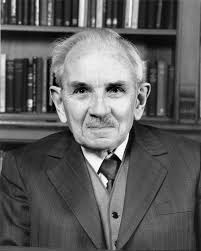
\includegraphics[height=3cm]{leray.jpg}
    \caption{Jean Leray (1906 -- 1998)}
\end{figure}

Em 1934, no artigo \textit{``Sur le mouvement d'un liquide visqueux emplassement l'espace''} (ver \cite{leray-fluid}) Leray construiu soluções fracas de energia finita\footnote{i.e., $\Vert \bu(\cdot,t) \Vert_{\cL^2(\bR^3)} < \infty$.}
\begin{equation} \label{eq:solucao-leray}
    \bu(\cdot,t) \in \cL^\infty\big([0,\infty), \cL^2_\sigma(\bR^3)\big) \cap \cC_w\left([0,\infty), \cL^2(\bR^3)\right) \cap \cL^2\big([0,\infty), \dot H^1(\bR^3)\big)\footnotemark
\end{equation}
para as seguintes equações de Navier-Stokes em $\bR^3$: 
\footnotetext{
    As definições desses espaços são dadas abaixo:
    \begin{itemize}[label=$\cdot$]
        \item $L^\infty\big([0,\infty), L^2_\sigma(\bR^3)\big)$ é o espaço das funções $\bu(\cdot,t) : [0,\infty) \to L^2(\bR^3)$ tal que $\nabla \cdot \bu =0$ e $\Vert \bu(\cdot,t) \Vert_{L^2(\bR^3)} < \infty$.
        \item $\cC_w\left([0,\infty), L^2(\bR^3)\right)$ é o espaço das funções $\bu(\cdot,t) : [0,\infty) \to L^2(\bR^3)$ fracamente contínuas.
        \item $L^2\big([0,\infty), \dot H^1(\bR^3)\big)$ é o espaço das funções $\bu(\cdot,t) : [0,\infty) \to \dot H^1(\bR^3)$ tal que
        \[
            \int_0^\infty \Vert \bu(\cdot,t) \Vert_{\dot H^1(\bR^3)}^2 \,dt < \infty.
        \]
    \end{itemize}
    \vspace{3pt}
}
\begin{equation} \label{eq:navierstokes}
    \left\{
        \begin{aligned}
        &\bu_t + \bu \cdot \nabla \bu + \nabla p = \nu \Delta\bu;\\
        &\nabla\cdot\bu = 0;\\
        &\bu(\cdot,0) = \bu_0 \in \cL^2_\sigma(\bR^3),
        \end{aligned}
    \right.
\end{equation}
onde $\nu > 0$ é constante e $\nabla \cdot \bu = \sum_{j=1}^3 \frac{\partial u_j}{\partial x_j}$.
Estas soluções são tais que $\Vert \bu(\cdot,t) - \bu_0 \Vert_{\cL^2(\bR^3)} \to 0$, quando $t \to 0^+$, e satisfazem a desigualdade de energia abaixo:
\begin{equation} \label{eq:desigualdade-de-energia}
    \Vert \bu(\cdot,t) \Vert_{\cL^2(\bR^3)}^2 \leqslant \Vert \bu(\cdot,t) \Vert_{L^2(\bR^3)}^2 + 2\nu \int_0^t \Vert D\bu(\cdot,s) \Vert_{\cL^2(\bR^3)}^2 \,ds \leqslant \Vert \bu_0 \Vert_{\cL^2(\bR^3)}^2,
\end{equation}
para todo $t > 0$.
A unicidade desas soluções ainda é um problema em aberto; porém, no mesmo artigo Leray mostrou que existe um instante de tempo $T_{**}$ tal que a solução $\bu$ se torna suave em $\bR^3 \times [T_{**}, \infty)$ e $\bu(\cdot,t) \in \cL^{\infty}_{\loc}\big( [T_{**}, \infty), H^k(\bR^3) \big)$\footnote{i.e., $\Vert \bu(\cdot,t) \Vert_{H^k(K)} < \infty$, onde $K \subseteq [T_{**},\infty)$ é compacto.} para cada $k \geqslant 0$.
Um problema importante que foi deixado em aberto por Leray no final de seu artigo diz respeito ao decaimento de energia em $L^2$ da solução de (\ref{eq:navierstokes}). Matematicamente, isto significa entender o que acontece com $\Vert \bu(\cdot,t) \Vert_{\cL^2(\bR^3)}$, quando $t \to \infty$. Leray suspeitava que
\[
    \Vert \bu(\cdot,t) \Vert_{\cL^2(\bR^3)} \to 0,
\]
quando $t \to \infty$. Uma demonstração para esse fato será apresentada no Teorema \ref{thm:problema-leray}.

Uma outra forma de estudar propriedades das soluções das equações de Navier-Stokes (\ref{eq:navierstokes}) é a partir das soluções $\bv(\cdot,t)$ do problema linearizado
\begin{equation} \label{eq:navier-stokes-linearizado}
    \left\{
        \begin{aligned}
        &\bv_t = \nu \Delta \bv;\\
        &\bv(\cdot,t_0) = \bu(\cdot,t_0),
    \end{aligned}
    \right.
\end{equation}
com $t \geqslant t_0 \geqslant 0$. Aqui, 
\[
    \bv(\cdot,t) = e^{\nu \Delta (t-t_0)} \bu(\cdot,t_0),
\]
onde $e^{\nu \Delta (t-t_0)}$ é o semigrupo do calor visto nos preliminares.
Com essas soluções, é possível estudar algumas estimativas de decaimento como
\[
    \Vert \bv(\cdot,t) \Vert_{\cL^2(\bR^n)} \to 0,
\]
\[
    t^{\frac{n}{4}}\Vert \bv(\cdot,t) \Vert_{\cL^\infty(\bR^n)} \to 0,
\]
\begin{equation} \label{eq:estimativa-sobolev-homogeneo}
    t^{\frac{s}{2}} \Vert \bv(\cdot,t) \Vert_{\dot H^s(\bR^n)} \to 0,
\end{equation}
quando $t \to \infty$,
onde $\dot H^s(\bR^n)$ é o espaço de Sobolev homogêneeo, formado pelas funções $\bv \in \cL^2(\bR^n)$, tais que $\Vert \cdot \Vert^s \, |\hat \bv(\cdot)| \in \cL^2$ e sua norma é dada por
\[
    \Vert \bv \Vert_{\dot H^s(\bR^n)} = \left( \int_{\bR^n} \Vert \omega \Vert^{2s} \, \Vert \hat \bv(\omega) \Vert^2 \,d\omega \right)^\frac{1}{2}.
\]
Uma outra pergunta importante (que não será trabalhada aqui) é sobre o erro ou diferença da solução de Leray e da solução do problema linearizado.
Essa pergunta foi respondida por Weigner (em \cite{wiegner-decay}), onde foi provado que
\[
    t^{\frac{n}{4} - \frac{1}{2}} \Vert \bu(\cdot,t) - e^{\nu \Delta (t-t_0)} \bu(\cdot,t_0) \Vert_{\cL^2(\bR^3)} \to 0,
\]
quando $t \to \infty$.

\subsection{Resultados auxiliares}

Tomando uma função molificadora $\eta \in \cC^{\infty}_c(\bR^3)$ e sua versão escalada $\eta_\delta$ (vista no Capítulo \ref{ch:sobolev}, Seção \ref{sec:aproximacoes}) definimos $\bar\bu_{0,\delta} = \eta_\delta * \bu_0$, introduzimos $\bu_\delta, p_\delta \in \cC^{\infty}\big( \bR^3 \times [0,\infty) \big)$ como a solução única do problema regularizado
\begin{equation} \label{eq:navier-stokes-regularizado}
    \left\{
        \begin{aligned}
        &\partial_t \bu_\delta + \bar \bu_\delta \cdot \nabla \bu_\delta  + \nabla p_\delta= \nu \Delta \bu_\delta;\\
        &\bu_\delta(\cdot,0) = \bar \bu_{0,\delta},
        \end{aligned}
    \right.
\end{equation}
onde $\bar\bu_\delta = \eta_\delta * \bu_\delta$. Em seu artigo, Leray mostrou que existe uma sequência apropriada $\delta' \to 0$ tal que conseguimos seguinte a convergência fraca\footnote{Dado um espaço de Banach $X$, dizemos que uma sequência $(x_n) \subseteq X$ converge fracamente para $x \in X$ ($x_n \rightharpoonup x$) se $f(x_n) \to f(x)$, para todo $f \in X'$, onde $X'$ é o espaço de todos funcionais lineares limitados de $X$ em $\bR$.} em $\cL^2(\bR^3)$:
\begin{equation} \label{eq:b1}
    \bu_{\delta'} \rightharpoonup \bu,
\end{equation}
para todo $t \geqslant 0$, onde $\bu(\cdot,t)$ apresentada em (\ref{eq:solucao-leray}) é contínua no instante $t = 0$.
Além disso, a desigualdade de energia (\ref{eq:desigualdade-de-energia}) é satisfeita para todo $t \geqslant 0$ e, em particular,
\begin{equation} \label{eq:2.3}
    \int_0^\infty \Vert D\bu_\delta(\cdot,t) \Vert_{\cL^2(\bR^3)}^2 \,dt \leqslant \frac{1}{2\nu} \Vert \bu_{0} \Vert_{\cL^2(\bR^3)}.
\end{equation}
Outros resultados importantes se referem à projeção de Helmholtz\footnote{A projeção de Helmholtz é uma forma de escrever um campo vetorial $F$ como $F = G + H$, onde $G, H$ são campos vetoriais tais que $\nabla \cdot G = 0$ e $H = \nabla \Phi$ para alguma função $\Phi : \bR^n \to \bR$.} de $-\bu(\cdot,t) \cdot \nabla \bu(\cdot,t)$ em $\cL^2_\sigma(\bR^3)$ isto é, o campo $\BQ(\cdot,t) \in \cL^2_\sigma(\bR^3)$ dado por
\begin{equation} \label{eq:defQ}
    \BQ(\cdot,t) := -\bu(\cdot,t) \cdot \nabla \bu(\cdot,t) - \nabla p(\cdot,t),
\end{equation}
para todo $t > 0$.
A seguir, estudaremos algumas estimativas para $\BQ(\cdot,t)$.

\begin{pbox} \label{pr:nsei}
    Para quase todo $s > 0$ (e para todo $s \geqslant T_{**}$), tem-se
    \[
        \Vert e^{\nu\Delta(t-s)}\BQ(\cdot,s) \Vert_{\cL^2(\bR^3)} \leqslant c \nu^{-\frac{3}{4}} (t-s)^{-\frac{3}{4}} \Vert \bu(\cdot,s) \Vert_{\cL^2(\bR^3)} \Vert D\bu(\cdot,s) \Vert_{\cL^2(\bR^3)},
    \]
    para todo $t > s$, onde $c$ é uma constante positiva.
\end{pbox}
\begin{prf}
    Seja $\hat f = \cF[f]$ a transformada de Fourier de uma função $f \in \cL^1(\bR^3)$, dada por
    \[
        \hat f (\omega) = (2\pi)^{-\frac{3}{2}} \int_{\bR^3} e^{-i\omega \cdot x} f(x) \, dx.
    \]
    Dada $\bv(\cdot,s) \in \cL^1 (\bR^3) \cap \cL^2(\bR^3)$ arbitrária, obtemos, pelo Teorema \ref{thm:norma-transformada}, que
    \[
        \Vert e^{\nu\Delta(t-s)} \bv(\cdot,s) \Vert_{\cL^2(\bR^3)}^2 = \Vert \cF [e^{\nu\Delta(t-s)} \bv(\cdot,s)] \Vert_{\cL^2(\bR^3)}^2 = \int_{\bR^3} e^{-2\nu \Vert \omega \Vert^2 (t-s)}\Vert \hat\bv(\omega,s) \Vert^2 \,d\omega,
    \]
    onde utlizamos o resultado sobre a transformada de Fourier do semigrupo do calor (ver Teorema \ref{thm:propriedades-semi-grupo-calor} \textbf{(c)}). Além disso, $\Vert \hat \bv(\omega,s) \Vert^2 \leqslant \Vert \hat\bv(\cdot,s) \Vert_{\cL^\infty(\bR^3)} = \sup\{ \Vert \hat\bv(\omega,s) \Vert \,; \omega \in \bR^3 \}$. Logo,
    \[
        \Vert e^{\nu\Delta(t-s)} \bv(\cdot,s) \Vert_{\cL^2(\bR^3)}^2 \leqslant \Vert \hat\bv(\cdot,s) \Vert_{\cL^\infty(\bR^3)} \int_{\bR^3} e^{-2\nu (t-s) \Vert \omega \Vert^2} d\omega,
    \]
    onde a integral do lado direito é uma Gaussiana, cujo resultado é $c \nu^{-\frac{3}{2}} (t - s)^{-\frac{3}{2}}$. Portanto, podemos escrever
    \begin{equation} \label{eq:2.7}
        \Vert e^{\nu\Delta(t-s)} \bv(\cdot,s) \Vert_{\cL^2(\bR^3)}\leqslant c \nu^{-\frac{3}{4}} (t-s)^{-\frac{3}{4}} \Vert \hat\bv(\cdot,s) \Vert_{\cL^\infty(\bR^3)}.
    \end{equation}
    O resultado que queremos, é uma aplicação direta de (\ref{eq:2.7}) com $\bv(\cdot,s) = \BQ(\cdot,s)$, o restante da demonstração será dedicado à estimativa do valor de $\Vert \hat\BQ(\cdot,s) \Vert_{\cL^\infty(\bR^3)}$. 
    
    Note que utilizando a derivada da transformada de Fourier, temos que $\cF[D^\alpha f] = (i\omega)^\alpha \hat f$ (ver Teorema \ref{thm:propriedades-transformada}), sendo assim se $\alpha = e_j$, para algum $j = 1,2,3$, $\cF [D^{e_j} f] = i\omega_j \hat f$. Dito isso,
    \[
        \cF[\nabla p(\cdot,s)] = i \hat p(\omega,s) \omega,
    \] 
    e $\omega \cdot \hat\BQ = 0$, pois, por (\ref{eq:defQ}) e (\ref{eq:navierstokes}), $\BQ = \bu_t - \nu \Delta \bu$ e 
    \[
        \nabla \cdot \BQ = (\nabla \cdot \bu)_t - \nu \Delta (\nabla \cdot \bu) = 0,
    \]
    já que $\nabla \cdot \bu = 0$. Dessa forma,
    \[
        0 = \widehat{\nabla \cdot \BQ} = \sum_{j=1}^3 \widehat{\frac{\partial Q_j}{\partial x_j}} = \sum_{j=1}^3 i \omega_j \hat Q_j,
    \] 
    ou seja, $\omega \cdot \hat\BQ = 0$. Além disso, pela definição de $\BQ(\cdot,s)$ (ver (\ref{eq:defQ})), temos que
    \[
        \hat\BQ(\omega,s) + \cF[\nabla p(\cdot,s)](\omega) = -\cF[\bu(\cdot,s) \cdot \nabla\bu(\cdot,s)](\omega).
    \]
    Com isso, fazendo o produto interno por $\hat\BQ$ em ambos os lados da igualdade acima, obtemos
    \[
        \hat\BQ(\omega,s) \cdot \hat\BQ(\omega,s) + i \hat p (\omega,s) \omega \cdot \hat\BQ(\omega,s) =  -\cF[\bu(\cdot,s) \cdot \nabla\bu(\cdot,s)](\omega) \cdot \hat\BQ(\omega,s)
    \]
    Deste modo, pela desigualde de Cauchy-Schwarz, podemos escrever,
    \[
        \Vert \hat\BQ(\omega,s) \Vert^2 \leqslant \Vert \cF [\bu(\cdot,s) \cdot \nabla \bu(\cdot,s)] \Vert \Vert \hat\BQ \Vert.
    \]
    Ou seja,
    \[
        \Vert \hat\BQ(\omega,s) \Vert \leqslant \Vert \cF[\bu(\cdot,s) \cdot \nabla\bu(\cdot,s)](\omega) \Vert.
    \]
    Isso nos diz que
    \begin{equation} \label{eq:2.9}
        \Vert \hat\BQ (\cdot,s) \Vert_{\cL^\infty(\bR^3)} \leqslant \Vert \cF [\bu \cdot \nabla \bu](\cdot,s) \Vert_{\cL^\infty(\bR^3)}.
    \end{equation}
    Por outro lado, para $i = 1,2,3$, é verdade que
    \[
        | \cF[\bu (\cdot,s) \cdot \nabla u_i(\cdot,s)](\omega)| \leqslant \sum_{j=1}^{3} | \cF[u_j (\cdot,s) D_j\, u_i(\cdot,s)](\omega)| \leqslant (2\pi)^{-\frac{3}{2}} \sum_{j=1}^3 \Vert u_j(\cdot,s) D_j\,u_i(\cdot,s) \Vert_{\cL^1(\bR^3)},
    \]
    para todo $\omega \in \bR^3$.
    Por fim, novamente utilizando a Desigualdade de Hölder (Cauchy-Schwarz) e a definição das normas, chegamos a
    \[
        | \cF[\bu (\cdot,s) \cdot \nabla u_j(\cdot,s)](\omega)| \leqslant c \Vert \bu(\cdot,s) \Vert_{\cL^2(\bR^3)} \Vert \nabla u_j(\cdot,s) \Vert_{\cL^2(\bR^3)},
    \]
    para todo $\omega \in \bR^3$.
    Isto mostra que
    \begin{equation} \label{eq:2.10}
        \Vert \cF[\bu\cdot \nabla \bu] (\cdot,s) \Vert_{\cL^\infty(\bR^3)} \leqslant c\Vert \bu(\cdot,s) \Vert_{\cL^2(\bR^3)} \Vert D \bu(\cdot,s) \Vert_{\cL^2(\bR^3)}.
    \end{equation}
    Dito isso, por (\ref{eq:2.7}), (\ref{eq:2.9}) e (\ref{eq:2.10}), inferimos que
    \[
        \Vert e^{\nu\Delta(t-s)}\BQ(\cdot,s) \Vert_{\cL^2(\bR^3)} \leqslant c \nu^{-\frac{3}{4}} (t-s)^{-\frac{3}{4}} \Vert \bu(\cdot,s) \Vert_{\cL^2(\bR^3)} \Vert D\bu(\cdot,s) \Vert_{\cL^2(\bR^3)},
    \]
    como queriamos mostrar.
\end{prf}

Repetindo o argumento utilizado na demonstração acima para as soluções do problema regularizado (\ref{eq:navier-stokes-regularizado}), obtemos
\begin{equation} \label{eq:2.11}
    \Vert e^{\nu\Delta(t-s)} \BQ_\delta \Vert_{\cL^2(\bR^3)} \leqslant c \nu^{-\frac{3}{4}}(t - s)^{-\frac{3}{4}} \Vert \bu_\delta(\cdot,s) \Vert_{\cL^2(\bR^3)} \Vert D\bu_\delta(\cdot,s) \Vert_{\cL^2(\bR^3)},
\end{equation}
onde $c$ é uma constante positíva e
\[
    \BQ_\delta(\cdot,s) = -\bar\bu_\delta(\cdot,s) \cdot \nabla \bu_\delta(\cdot,s) - \nabla p_\delta(\cdot,s).
\]

\obs Vale ressaltar que as soluções do problema regularizado também satisfazem a seguinte desigualdade de energia:
\begin{equation} \label{eq:desigualdade-de-energia-regularizado}
    \Vert \bu_\delta(\cdot,t) \Vert_{\cL^2(\bR^3)}^2 + 2\nu \int_0^t \Vert D\bu_\delta(\cdot,s) \Vert^2_{\cL^2(\bR^3)} \,ds \leqslant \Vert \bu_0 \Vert_{\cL^2(\bR^3)}^2,
\end{equation}
para todo $t > 0$.

O resultado a seguir é uma generalização da Proprosição \ref{pr:nsei}.

\begin{pbox} \label{pr:DaQ}
    Para quase todo $s > 0$ (e todo $s \geqslant T_{**}$), tem-se
    \[
        \Vert D^{\alpha} \big( e^{\nu\Delta(t-s)}\BQ(\cdot,s)\big) \Vert_{\cL^2(\bR^3)} \leqslant c(k) \nu^{-\left( \frac{k}{2} + \frac{3}{4} \right)} (t - s)^{-\left( \frac{k}{2} + \frac{3}{4}\right)} \Vert \bu(\cdot,s) \Vert_{\cL^2(\bR^3)} \Vert D\bu(\cdot,s) \Vert_{\cL^2(\bR^3)},
    \]
    para todo $t > s$, onde $k = |\alpha|$ e $c(k)$ depende apenas de $k$.
\end{pbox}
\begin{prf}
    Por (\ref{eq:estimativa-util}), obtemos
    \[
        \begin{aligned}
            \Vert D^\alpha [e^{\nu \Delta (t - s)} \BQ(\cdot,s)] \Vert_{\cL^2(\bR^3)} &= \Vert D^\alpha \big[e^{\nu \Delta (t - s)/2} [ e^{\nu \Delta (t - s)/2} \BQ(\cdot,s) ] \big] \Vert_{\cL^2(\bR^3)}\\ 
            &\leqslant c(k) \nu^{-\frac{k}{2}} (t - s)^{-\frac{k}{2}} \Vert e^{\nu\Delta(t-s)/2} \BQ(\cdot,s) \Vert_{\cL^2(\bR^3)},
        \end{aligned}
    \]
    e, pela Proposição \ref{pr:nsei}, podemos escrever
    \[
        \Vert D^\alpha [e^{\nu \Delta (t - s)/2} \BQ(\cdot,s)] \Vert_{\cL^2(\bR^3)} \leqslant c(k) \nu^{-\left( \frac{k}{2} + \frac{3}{4} \right)} (t - s)^{-\left( \frac{k}{2} + \frac{3}{4} \right)} \Vert \bu(\cdot,s) \Vert_{\cL^2(\bR^3)} \Vert D\bu(\cdot,s) \Vert_{\cL^2(\bR^3)}.
    \]
\end{prf}

A seguir, mostremos que o gradiente da solução de Leray se torna decrescente a partir de um instante de tempo.

\begin{pbox} \label{pr:tstar}
    Seja $\bu(\cdot,t)$ uma solução de Leray para (\ref{eq:navierstokes}). Então existe $t_{**} > T_{**}$ (com $t_{**}$ dependendo da solução $\bu$) suficientemente grande tal que $\Vert D\bu(\cdot,t) \Vert_{\cL^2(\bR^3)}$ é uma funçao monotonicamente decrescente de $t$ no intervalo $[t_{**}, \infty)$.
\end{pbox}
\begin{prf}
    Sejam $t_0 \geqslant T_{**}$ e $t > t_0$.
    Aplicando a $k$-ésima derivada parcial $D_k$ à primeira equação de (\ref{eq:navierstokes}), realizando o produto escalar com $D_k \bu$, integrando em $\bR^3 \times [t_0,t]$, obtemos
    \begin{equation} \label{eq:A}
        \begin{aligned}
            \int_{\bR^3} \int_{t_0}^t D_k \bu_s \cdot D_k \bu \,dsdx &+ \int_{\bR^3} \int_{t_0}^t D_k (\bu \cdot \nabla \bu) \cdot D_k \bu \,dsdx\\ 
            &+ \int_{\bR^3} \int_{t_0}^t D_k (\nabla p) \cdot D_k\bu \,dsdx = \nu \int_{\bR^3} \int_{t_0}^t D_k (\Delta \bu) \cdot D_k \bu \,dsdx
        \end{aligned}
    \end{equation}
    Vamos analisar cada integral separadamente.
    Note que
    \[
        D_k \bu_t \cdot D_k \bu = \frac{1}{2} \frac{d}{dt} \Vert D_k \bu \Vert^2.
    \]
    Dessa forma 
    \[
        \int_{t_0}^t D_k \bu_s \cdot D_k \bu \,dsdx = \int_{t_0}^t \frac{1}{2} \frac{d}{ds} \Vert D_k \bu(\cdot,s) \Vert^2 \,dx =  \frac{1}{2} \big[ \Vert D_k \bu(\cdot,t) \Vert^2 -  \Vert D_k \bu(\cdot,t_0) \Vert^2 \big] .
    \]
    Além disso, a segunda integral em (\ref{eq:A}) pode ser estudada da seguinte forma
    \begin{align}
            \int_{\bR^3} D_k (\bu \cdot \nabla \bu) \cdot D_k \bu \,dx &= \sum_{i,j=1}^3 \int_{\bR^3} D_k (u_i D_i u_i) D_k u_j \,dx \label{eq:xx1}\\
            &= \sum_{i,j=1}^3 \int_{\bR^3} (D_k u_i) (D_i u_j)(D_k u_j) \,dx + \sum_{i,j=1}^3 \int_{\bR^3} u_i (D_k D_i u_j) (D_k u_j)\,dx. \nonumber
    \end{align}
    Por outro lado, utilizando integração por partes (ver Teorema \ref{thm:integracao-por-partes}) inferimos que
    \[
        \begin{aligned}
            \sum_{i,j=1}^3 \int_{\bR^3} u_i (D_k D_i u_j)(D_k u_j) \,dx &= -\sum_{i,j=1}^3 \int_{\bR^3} (D_i u_i) (D_k u_j)^2 \,dx - \sum_{i,j=1}^{3} \int_{\bR^3} u_i (D_k u_j) (D_k D_i u_j) \,dx\\
            &=-\sum_{j=1}^3 \int_{\bR^3} (\nabla \cdot \bu) (D_k u_j)^2 \,dx - \sum_{i,j=1}^3 \int_{\bR^3} u_i D(D_k D_i u_j) (D_k u_j) \,dx\\
            &=- \sum_{i,j=1}^3 \int_{\bR^3} u_i D(D_k D_i u_j) (D_k u_j) \,dx,
        \end{aligned}
    \]
    pois $\nabla \cdot \bu = 0$. Ou seja
    \begin{equation} \label{eq:x2}
        \sum_{i=1}^3 \sum_{j=1}^{3} \int_{\bR^3} u_i (D_k D_i u_j) (D_k u_j) \,dx = 0.
    \end{equation}
    Análogamente, podemos escrever
    \begin{align}
        \sum_{i,j=1}^3 \int_{\bR^3} (D_k u_i) (D_i u_j) (D_k u_j) \,dx &= -\sum_{j=1}^{3} \int_{\bR^3} D_k (\nabla \cdot \bu) u_j (D_k u_j) \,dx - \sum_{i,j=1}^3 \int_{\bR^3} (D_k u_j) I_k D_i D_k u_j \,dx \nonumber\\
        &= - \sum_{i,j=1}^3 \int_{\bR^3} (D_k u_j) u_k D_i D_k u_j \,dx. \label{eq:x3}
    \end{align}
    Substituindo (\ref{eq:x2}) e (\ref{eq:x3}) em (\ref{eq:xx1}), chegamos a
    \[
        \int_{\bR^3} D_k(\bu \cdot \nabla \bu) \,dx = - \sum_{i,j=1}^{3} \int_{\bR^3} u_j (D_k u_i) (D_i D_k u_j) \,dx.
    \]
    A terceira integral em (\ref{eq:A}) é nula, já que
    \[
        \int_{\bR^3} D_k (\nabla p) \cdot D_k \bu \,dx = \sum_{j=1}^{3} \int_{\bR^3} D_k D_j p D_k u_j \,dx,
    \]
    e, utlizando integração por partes (ver Teorema \ref{thm:integracao-por-partes}), obtemos
    \[
        \int_{\bR^3} D_k \nabla p \cdot D_k \bu \,dx = -\sum_{j=1}^3 \int_{\bR^3} D_k p D_j D_k  u_j \,dx = - \int_{\bR^3} D_k p D_k \left( \bu \cdot \nabla \bu \right) \,dx = 0,
    \]
    pois novamente $\nabla \cdot \bu = 0$.
    Por fim, a última integral em (\ref{eq:A}) pode ser escrita da seguinte forma:
    \[
        \int_{\bR^3} \Delta D_k \bu \cdot D_k \bu \,dx = \sum_{i,j=1}^3 \int_{\bR^3} D_j^2 D_k u_i D_k u_i 
    \]
    novamente utilizando integração por partes, concluimos que
    \[
        \begin{aligned}
            \int_{\bR^3} \Delta D_k \bu \cdot D_k \bu \,dx &= -\sum_{i,j=1}^3 \int_{\bR^3} (D_jD_k u_i)(D_jD_k u_i)\\ 
            &= -\sum_{i,j=1}^3  \int_{\bR^3} (D_j D_k u_i)^2 \,dx = -\!\!\int_{\bR^3} \Vert D_kD\bu \Vert^2 \,dx
        \end{aligned}
    \]
    Dito isso, voltando para (\ref{eq:A}) e somando em $1 \leqslant k \leqslant 3$, segue que
    \[
        \begin{aligned}
            \frac{1}{2} \sum_{k=1}^3 \int_{\bR^3} \Vert D_k \bu(\cdot,t) \Vert^2 - \Vert D_k \bu(\cdot,t_0) \Vert^2 \,dx  &+ \nu \sum_{k=1}^3 \int_{t_0}^t \int_{\bR^3} \Vert D_kD\bu \Vert^2 \,dx ds\\
        &= \sum_{i=1}^3 \sum_{j=1}^3\sum_{k=1}^3 \int_{t_0}^{t}\int_{\bR^3} u_j D_k u_i D_i D_k u_j \,dxds.
        \end{aligned}
    \]
    Lembrando da definição das normas vistas nos preliminares, multiplicando ambos os lados por $2$ e reorganizando os termos, deduzimos que
    \begin{equation} \label{eq:y2}
        \begin{aligned}
            \Vert D\bu(\cdot,t) \Vert_{\cL^2(\bR^3)}^2 &+ 2\nu \int_{t_0}^t \Vert D^2 \bu(\cdot,t) \Vert_{\cL^2(\bR^3)}^2 \,ds\\ &= \Vert D\bu(\cdot,t_0) \Vert_{\cL^2(\bR^3)}^2 + 2 \sum_{i=1}^3 \sum_{j=1}^3\sum_{k=1}^3 \int_{t_0}^t \int_{\bR^3} u_i D_k u_j D_j D_k u_i \,dxds.
        \end{aligned}
    \end{equation}
    Vamos análisar o último termo da equação acima separadamente.
    Note que utilizando a desigualdade de Hölder (ver Teorema \ref{thm:pre-desigualdade-de-holder}) e as definições das normas, temos que
    \[
        \begin{aligned}
            \sum_{i=1}^3\sum_{j=1}^3\sum_{k=1}^3 \int_{\bR^3} u_i (D_k u_j)(D_k D_k u_i)\,dx &= \sum_{j=1}^3 \sum_{k=1}^3 \int_{\bR^3} (D_k u_j) \left( \sum_{i=1}^3 u_i (D_j D_k u_i) \right) \,dx\\
            &\leqslant \sum_{j=1}^3 \sum_{k=1}^{3} \int_{\bR^3} (D_k u_j) \left( \sum_{i=1}^3 u_i^2      \right)^{\frac{1}{2}} \left( \sum_{i=1}^3 (D_j D_k u_i)^2 \right)^{\frac{1}{2}} \,dx\\
            &=\sum_{j=1}^3\sum_{k=1}^{3} \int_{\bR^3} (D_k u_j) \Vert \bu \Vert \Vert D_j D_k \bu \Vert \,dx.
        \end{aligned}
    \]
    Novamente utilizando a desigualdade de Hölder, obtemos
    \[
        \begin{aligned}
            \sum_{i=1}^3\sum_{j=1}^3\sum_{k=1}^3 \int_{\bR^3} u_i (D_k u_j)(D_k D_k u_i)\,dx
            &\leqslant \Vert \bu \Vert_{\cL^\infty(\bR^3)} \sum_{j=1}^3 \int_{\bR^3} \left( \sum_{k=1}^3 |D_k u_j|^2 \right)^{\frac{1}{2}} \left( \sum_{k=1}^3 \Vert D_j D_k \bu \Vert \right)^{\frac{1}{2}} \,dx\\
            &\leqslant \Vert \bu \Vert_{\cL^\infty(\bR^3)} \sum_{j=1} \int_{\bR^3} \Vert Du_j \Vert \Vert D_j D\bu \Vert \,dx.
        \end{aligned}
    \]
    Utilizando a desigualdade de Hölder mais uma vez, segue que
    \[
        \begin{aligned}
            \sum_{i=1}^3\sum_{j=1}^3\sum_{k=1}^3 \int_{\bR^3} u_i (D_k u_j)(D_k D_k u_i)\,dx &\leqslant \Vert \bu \Vert_{\cL^\infty(\bR^3)}\int_{\bR^3} \left( \sum_{j=1}^3 \Vert D u_j \Vert^2 \right)^{\frac{1}{2}} \left( \sum_{j=1}^{3} \Vert Dj D\bu \Vert^2  \right)^{\frac{1}{2}} \,dx\\
            &=\Vert \bu \Vert_{\cL^\infty(\bR^3)} \int_{\bR^3} \Vert D\bu \Vert \Vert D^2 \bu \Vert \,dx.
        \end{aligned}
    \]
    Ainda utilizando a desigualdade de Hölder, concluimos que
    \begin{equation} \label{eq:y1}
        \begin{aligned}
            \sum_{i=1}^3\sum_{j=1}^3\sum_{k=1}^3 \int_{\bR^3} u_i (D_k u_j)(D_k D_k u_i)\,dx &\leqslant \Vert \bu \Vert_{\cL^2} \left( \int_{\bR^3} \Vert D\bu \Vert^2 \right)^{\frac{1}{2}} \left( \int_{\bR^3}  \Vert D^2\bu \Vert^{2} \right)^{\frac{1}{2}}\\ 
            &= \Vert \bu \Vert_{\cL^\infty(\bR^3)} \Vert D\bu \Vert_{\cL^2(\bR^3)} \Vert D^2 \bu \Vert_{\cL^2(\bR^3)}.
        \end{aligned}
    \end{equation}
    Portanto, substituindo (\ref{eq:y1}) em (\ref{eq:y2}), chegamos a
    \[
        \begin{aligned}
            \Vert D\bu(\cdot,t) \Vert_{\cL^2(\bR^3)}^2 &+ 2\nu \int_{t_0}^t \Vert D^2 \bu(\cdot,t) \Vert_{\cL^2(\bR^3)}^2 \,ds\\ &\leqslant \Vert D\bu(\cdot,t_0) \Vert_{\cL^2(\bR^3)}^2 + 2 \Vert \bu \Vert_{\cL^\infty(\bR^3)} \Vert D\bu \Vert_{\cL^2(\bR^3)} \Vert D^2 \bu \Vert_{\cL^2(\bR^3)},
        \end{aligned}
    \]
    que pela Desigualdade de Gagliardo-Nirenberg (\ref{eq:gagliardoinf}) em $\Vert \bu(\cdot,s) \Vert_{\infty}$, podemos escrever como:
    \[
        \begin{aligned}
            \Vert D\bu(\cdot,t) \Vert_{\cL^2(\bR^3)}^2 &+ 2\nu \int_{t_0}^t \Vert D^2 \bu(\cdot,t) \Vert_{\cL^2(\bR^3)}^2 \,ds\\ &\leqslant \Vert D\bu(\cdot,t_0) \Vert_{\cL^2(\bR^3)}^2 + 2 \! \int_{t_0}^t \Vert \bu(\cdot,s) \Vert_{\cL^2(\bR^3)}^{\frac{1}{2}} \Vert D\bu(\cdot,s) \Vert_{\cL^2(\bR^3)}^{\frac{1}{2}} \Vert D^2\bu(\cdot,s) \Vert_{\cL^2(\bR^3)}^2 \,ds.
        \end{aligned}
    \]
    Consequentemente, por (\ref{eq:desigualdade-de-energia}), podemos escrever
    \begin{align} 
        \Vert D\bu(\cdot,t) \Vert_{\cL^2(\bR^3)}^2 &+ 2 \nu \int_{t_0}^t \Vert D^2 \bu(\cdot,s) \Vert_{\cL^2(\bR^3)}^2 \,ds \label{eq:maisumadesigualdade}\\ &\leqslant \Vert D\bu(\cdot,t_0) \Vert_{\cL^2(\bR^3)}^2 + 2 \! \int_{t_0}^t \big[ \Vert \bu_0 \Vert_{\cL^2(\bR^3)} \Vert D\bu(\cdot,s) \Vert_{\cL^2(\bR^3)} \big]^\frac{1}{2} \Vert D^2\bu(\cdot,s) \Vert_{\cL^2(\bR^3)}^2, \nonumber
    \end{align}
    para todo $t \geqslant t_0$. 

    Seja $t_0 \geqslant T_{**}$ tal que
    \begin{equation} \label{eq:MM1}
        \Vert \bu_0 \Vert_{\cL^2(\bR^3)} \Vert D\bu(\cdot,t_0) \Vert_{\cL^2(\bR^3)} < \nu^2.
    \end{equation}
    Caso contrário,
    \[
        \Vert \bu_0 \Vert_{\cL^2(\bR^3)} \Vert D\bu(\cdot,s) \Vert_{\cL^2(\bR^3)} \geqslant \nu^2,
    \]
    para todo $s \geqslant T_{**}$.
    Integrando em $[T_{**},t]$, com $t \geqslant T_{**}$, teriamos
    \[
        \Vert \bu_0 \Vert_{\cL^2(\bR^3)} \int_{T_{**}}^{t} \Vert D\bu(\cdot,s) \Vert_{\cL^2(\bR^3)}^2 \geqslant  (t - T_{**})\nu^4,
    \]
    para todo $t \geqslant T_{**}$.
    Pela desigualdade de energia (\ref{eq:desigualdade-de-energia}), chegmos a
    \[
        t - T_{**} \leqslant \frac{\Vert \bu_0 \Vert_{\cL^2(\bR^3)}^2}{2 \nu^5},
    \]
    para todo $t \geqslant T_{**}$.
    Isto é um absurdo, pois estariamos dizendo que $t$ possui cota superior.
    Dessa forma, afirmamos que
    \begin{equation} \label{eq:MM2}
        \Vert \bu_0 \Vert_{\cL^2(\bR^3)} \Vert D\bu(\cdot,s) \Vert_{\cL^2(\bR^3)} < \nu^2,
    \end{equation}
    para todo $s \geqslant t_0$.
    Com efeito, se (\ref{eq:MM2}) não fosse válida, por suavidade existiria $t_1 > t_0$ tal que
    \begin{equation} \label{eq:MM3}
        \Vert \bu_0 \Vert_{\cL^2(\bR^3)} \Vert D\bu(\cdot,s) \Vert_{\cL^2(\bR^3)} < \nu^2,
    \end{equation}
    para todo $t_0 \leqslant s < t_1$, com
    \begin{equation} \label{eq:MM4}
        \Vert \bu_0 \Vert_{\cL^2(\bR^3)} \Vert D\bu(\cdot,t_1) \Vert_{\cL^2(\bR^3)} = \nu^2.
    \end{equation}
    \begin{figure}
        \centering
        \begin{tikzpicture}[scale=0.9]
            % \draw[black!10] (0,0) grid (11,5);

            \draw[ultra thick, tangerine!80!black]
            (3.39,2.54) .. controls (1.46,-2.68) and (1.64,3) .. (0.00,3);

            \draw[ultra thick, tangerine!80!black]
            (3.39,2.54) .. controls (5.32,7.76) and (5.72,1.00) .. (10.32,1.00);
            
            \draw[dashed, black!30] (0,4) to (11,4);
            \draw[dashed, black!30] (0,1.58) to (11,1.58);

            
            \draw[black!80, -stealth] (0,-0.5) to (0,5);
            \draw[black!80, -stealth] (-2,0) to (11,0);

            \draw[dashed, black!30] (4.071,4) to (4.071,0);
            \draw[dashed, black!30] (3,1.58) to (3,0);

            \node[anchor=east] at (0,4) {$\phi(t_1) = \nu^2$};
            \node[anchor=east] at (0,1.58) {$\phi(t_0)$};

            \node[anchor=north] at (3,0) {$t_0$};
            \node[anchor=north] at (4.071,0) {$t_1$};

            \node[anchor=west] at (11,0) {$s$};
            \node[anchor=west] at (0,4.8) {$\phi(s)$};
        \end{tikzpicture}
        \caption{Representação visual de (\ref{eq:MM3}) e (\ref{eq:MM4}), onde $\phi(s) = \Vert \bu_0 \Vert_{\cL^2(\bR^3)} \Vert D\bu(\cdot,s) \Vert_{\cL^2(\bR^3)}$.\\Fonte: Autoral.}
    \end{figure}
    Escolhendo $t=t_1$ em (\ref{eq:maisumadesigualdade}), temos que
    \[
        \Vert D\bu(\cdot,t_1) \Vert_{\cL^2(\bR^3)} \leqslant \Vert D\bu(\cdot,t_0) \Vert_{\cL^2(\bR^3)}.
    \]
    De fato, por (\ref{eq:MM3}) e (\ref{eq:maisumadesigualdade}), podemos escrever
    \[
        \begin{aligned}
            \Vert D\bu(\cdot,t_1) \Vert_{\cL^2(\bR^3)}^2 &+ 2\nu \int_{t_0}^{t_1} \Vert D^2\bu(\cdot,s) \Vert_{\cL^2(\bR^3)}^2 \,ds\\
            &\leqslant \Vert D\bu(\cdot,t_0) \Vert_{\cL^2(\bR^3)}^2 + 2 \int_{t_0}^{t_1} \big[ \Vert \bu_0 \Vert_{\cL^2(\bR^3)}\Vert D\bu(\cdot,s) \Vert_{\cL^2(\bR^3)} \big]^{\frac{1}{2}} \Vert D^2\bu(\cdot,s) \Vert_{\cL^2(\bR^3)}^2\\
            &\leqslant \Vert D\bu(\cdot,t_0) \Vert_{\cL^2(\bR^3)}^2 + 2\nu \int_{t_0}^{t_1} \Vert D^2\bu(\cdot,s) \Vert_{\cL^2(\bR^3)}^2 \,ds,
        \end{aligned}
    \]
    o que resulta em
    \[
        \Vert D\bu(\cdot,t_1) \Vert_{\cL^2(\bR^3)} \leqslant \Vert D\bu(\cdot,t_0) \Vert_{\cL^2(\bR^3)},
    \]
    como era desejado. Então por (\ref{eq:MM4}) e (\ref{eq:MM1}), concluimos que
    \[
        \nu^2 = \Vert \bu_0 \Vert_{\cL^2(\bR^3)} \Vert D\bu(\cdot,t_1) \Vert_{\cL^2(\bR^3)} \leqslant \Vert \bu_0 \Vert_{\cL^2(\bR^3)} \Vert D\bu(\cdot,t_0) \Vert_{\cL^2(\bR^3)} < \nu^2,
    \]
    o que é uma contradição! Dessa forma, (\ref{eq:MM3}) é válida.
    Por (\ref{eq:maisumadesigualdade}) e (\ref{eq:MM1}), inferimos que
    \[
        \begin{aligned}
            \Vert D\bu(\cdot,t) \Vert_{\cL^2(\bR^3)}^2 &+ 2\nu \int_{t_0}^t \Vert D^2 \bu(\cdot,s) \Vert_{\cL^2(\bR^3)}^2 \,ds\\
            &\leqslant \Vert D\bu(\cdot,t_0) \Vert_{\cL^2(\bR^3)}^2 + 2\nu \int_{t_0}^t \Vert D^2 \bu(\cdot,s) \Vert_{\cL^2(\bR^3)} \,ds,
        \end{aligned}
    \]
    pra todo $t \geqslant t_0$. Com isso,
    \begin{equation} \label{eq:MM5}
        \Vert D\bu(\cdot,t) \Vert_{\cL^2(\bR^3)} \leqslant \Vert D\bu(\cdot,t_0) \Vert_{\cL^2(\bR^3)},
    \end{equation}
    para todo $t \geqslant t_0$.
    Pela prova de (\ref{eq:maisumadesigualdade}) e por (\ref{eq:MM5}), deduzimos que
    \[
        \begin{aligned}
            \Vert D\bu(\cdot,t) \Vert_{\cL^2(\bR^3)}^2 & \leqslant \Vert D\bu(\cdot,t) \Vert_{\cL^2(\bR^3)}^2 + 2 \gamma \int_{t_2}^t \Vert D^2\bu(\cdot,s) \Vert_{\cL^2(\bR^3)}^2 \,ds \leqslant \Vert D\bu(\cdot,t_2) \Vert_{\cL^2(\bR^3)}^2,
        \end{aligned}
    \]
    para todo $t \geqslant t_2 \geqslant t_0$, onde $\gamma = \nu - \Vert \bu_0 \Vert_{\cL^2(\bR^3)}^{\frac{1}{2}} \Vert D\bu(\cdot,t_0) \Vert_{\cL^2(\bR^3)}^{\frac{1}{2}} > 0$ é uma constante.
    Portanto, escolhendo $t_{**} = t_2$, finalizamos a demonstração, pois mostrmos que
    \[
        \Vert D\bu(\cdot,t) \Vert_{\cL^2(\bR^3)} \leqslant \Vert D\bu(\cdot,t_2) \Vert_{\cL^2(\bR^3)},
    \]
    para todo $t \geqslant t_{**}$.
\end{prf}

A proposição abaixo utiliza a solução do problema linearizado (\ref{eq:navier-stokes-linearizado}) para estabelecer uma estimativa importante para o prosseguimento do nosso texto.

\begin{pbox} \label{pr:dav}
    Seja $\bu(\cdot,t)$ solução de Leray para (\ref{eq:navierstokes}).
    Dados $\tilde t_0 > t_0 > 0$, tem-se
    \[
        \Vert D^\alpha \bv(\cdot,t) - D^\alpha \tilde \bv(\cdot,t)\Vert_{\cL^2(\bR^3)} \leqslant c(k) \nu^{-\left( \frac{5}{4} + \frac{k}{2} \right)} \Vert \bu_0 \Vert_{\cL^2(\bR^3)}^2 (\tilde t_0 - t_0)^{\frac{1}{2}} (t - \tilde t_0)^{-\left( \frac{3}{4} + \frac{k}{2} \right)},
    \]
    para todo $t > \tilde t_0$, onde $\bv(\cdot,t) = e^{\nu\Delta(t-t_0)} \bu(\cdot,t_0)$, $\tilde\bv(\cdot,t) = e^{\nu\Delta(t-\tilde t_0)} \bu(\cdot,\tilde t_0)$ e $k = |\alpha|$.
\end{pbox}
\begin{prf}
    Primeiramente, reescrevemos $\bv(\cdot,t)$ como
    \[
        \bv(\cdot,t) = e^{\nu\Delta(t-t_0)} \left[\bu(\cdot,t_0) - \bu_\delta(\cdot,t_0)\right] + e^{\nu\Delta(t-t_0)}\bu_\delta(\cdot,t_0),
    \]
    onde $t > t_0$ e $\bu_\delta(\cdot,t)$ é dada em (\ref{eq:navier-stokes-regularizado}).
    Ademais, temos que
    \begin{equation} \label{eq:5}
        \bu_\delta(\cdot,t_0) = e^{\nu\Delta t_0}\bar\bu_{0,\delta} + \int_0^{t_0} e^{\nu\Delta(t_0 - s)}\BQ_\delta(\cdot,s)\,ds.
    \end{equation}
    Com efeito, considere a equação
    \[
        \partial_t \bu_\delta = \BQ_\delta + \nu\Delta\bu_\delta,
    \]
    onde $\BQ_\delta = - \bar\bu_\delta \cdot \nabla \bu_\delta - \nabla p_\delta$ e $\bar{\bu}_\delta = \eta_\delta * \bar{\bu}_\delta$.
    Aplique o semigrupo do calor $e^{\nu\Delta(t_0 - s)}$ em ambos os lados e integre sobre $[0,t_0]$ para obter
    \begin{equation} \label{eq:4}
        \int_0^{t_0} e^{\nu\Delta(t_0 - s)} \partial_s \bu_\delta \,ds = \int_0^{t_0} e^{\nu\Delta(t_0 - s)}\BQ_\delta \,ds + \nu\int_0^{t_0} e^{\nu\Delta(t_0 - s)} \Delta \bu_\delta \, ds.
    \end{equation}
    Além disso, note que
    \[
        \partial_s \left[ e^{\nu\Delta(t_0-s)}\bu_\delta \right] = -\nu e^{\nu\Delta(t_0 -s)}\Delta\bu_\delta + e^{\nu\Delta(t_0 - s)} \partial_s \bu_\delta,
    \]
    ou seja,
    \[
        e^{\nu\Delta(t_0 - s)} \partial_s \bu_\delta = \partial_s \left[ e^{\nu\Delta(t_0-s)}\bu_\delta \right] + \nu e^{\nu\Delta(t_0 -s)}\Delta\bu_\delta.
    \]
    Dessa forma, (\ref{eq:4}) se torna
    \[
        \int_0^{t_0}  \partial_s \left[ e^{\nu\Delta(t_0-s)}\bu_\delta \right] \,ds + \nu \int_0^{t_0} e^{\nu\Delta(t_0 -s)}\Delta\bu_\delta \,ds = \int_0^{t_0} e^{\nu\Delta(t_0 - s)}\BQ_\delta \,ds + \nu\int_0^{t_0} e^{\nu\Delta(t_0 - s)} \Delta \bu_\delta \,ds,
    \]
    isto é,
    \[
        \bu_\delta(\cdot,t_0) - e^{\nu \Delta t_0} \bar\bu_{0,\delta} = \int_0^{t_0} e^{\nu\Delta(t_0 - s)}\BQ_\delta \,ds,
    \]
    por (\ref{eq:navierstokes}). Isto prova (\ref{eq:5}).
    Dito isso, é verdade que
    \[
        \bv(\cdot,t) = e^{\nu\Delta(t - t_0)} \left[ \bu(\cdot,t_0) - \bu_\delta(\cdot,t_0) \right] + e^{\nu\Delta t}\bar\bu_{0,\delta} + \int_0^{t_0} e^{\nu\Delta(t-s)} \BQ_\delta(\cdot,s)\,ds,
    \]
    para todo $t>t_0$. De forma análoga, deduzimos que
    \[
        \tilde\bv(\cdot,t) = e^{\nu\Delta(t - \tilde t_0)} \left[ \bu(\cdot,\tilde t_0) - \bu_\delta(\cdot,\tilde t_0) \right] + e^{\nu\Delta t}\bar\bu_{0,\delta} + \int_0^{\tilde t_0} e^{\nu\Delta(t-s)} \BQ_\delta(\cdot,s)\,ds.
    \]
    para todo $t > \tilde t_0$.
    Dessa forma, podemos escrever
    \[
        \begin{aligned}
            D^\alpha\tilde\bv(\cdot,t) -  D^\alpha\bv(\cdot,t) &= D^\alpha\left( e^{\nu\Delta(t-\tilde t_0)} \big[\bu(\cdot,\tilde t_0) - \bu_\delta(\cdot,\tilde t_0)\big] \right)\\ 
            &- D^\alpha\left( e^{\nu\Delta(t-t_0)} \big[\bu(\cdot, t_0) - \bu_\delta(\cdot, t_0)\big] \right)
            + D^\alpha\int_{t_0}^{\tilde t_0} e^{\nu\Delta(t-s)}\BQ_{\delta}(\cdot,s) \,ds.
        \end{aligned}
    \]
    Agora, considere que $K \subseteq \bR^3$ é um compacto qualquer. Portanto, para cada $t > \tilde t_0$ e $\delta > 0$, infere-se
    \begin{equation} \label{eq:acima}
        \Vert D^\alpha\tilde\bv(\cdot,t) -  D^\alpha\bv(\cdot,t) \Vert_{\cL^2(K)} \leqslant J_{\alpha,\delta}(t) + \int_{t_0}^{\tilde t_0} \Vert D^\alpha\big[ e^{\nu\Delta(t-s)}\BQ_{\delta}(\cdot,s)\big] \Vert_{\cL^2(K)}\,ds,
    \end{equation}
    onde
    \[
        \begin{aligned}
            J_{\alpha,\delta}(t) = \big\Vert D^\alpha\big( e^{\nu\Delta(t-\tilde t_0)} \big[\bu(\cdot,\tilde t_0) &- \bu_\delta(\cdot,\tilde t_0)\big] \big) \big\Vert _{\cL^2(K)} \\
            &+ \big\Vert D^\alpha\big( e^{\nu\Delta(t-t_0)} \big[\bu(\cdot, t_0) - \bu_\delta(\cdot, t_0)\big] \big) \big\Vert _{\cL^2(K)}.
        \end{aligned}
    \]
    Utilizando a Proposição \ref{pr:DaQ} e (\ref{eq:2.11}), temos que
    \[
        \Vert D^\alpha\tilde\bv(\cdot,t) -  D^\alpha\bv(\cdot,t) \Vert_{\cL^2(K)} \leqslant J_{\alpha,\delta}(t) + c(k) \nu^{-\frac{k}{2}}\int_{t_0}^{\tilde t_0} (t - s)^{-\frac{k}{2}} \Vert e^{\nu\Delta(t-s)/2}\BQ_{\delta}(\cdot,s) \Vert_{\cL^2(\bR^3)} \,ds
    \]
    \begin{equation} \label{eq:3.3}
        \leqslant J_{\alpha,\delta}(t) + c(k) \nu^{-\left( \frac{k}{2} + \frac{3}{4} \right)} (t - \tilde t_0)^{-\frac{k}{2}} \int_{t_0}^{\tilde t_0} (t-s)^{-\frac{3}{4}} \Vert \bu_\delta(\cdot,s) \Vert_{\cL^2(\bR^3)} \Vert D\bu_\delta(\cdot,s) \Vert_{\cL^2(\bR^3)} \,ds.
    \end{equation}
    Observe que a integral acima pode ser simplificada, já que $s \leqslant \tilde t_0$ implica em $(t - s)^{-\frac{3}{4}} \leqslant (t - \tilde t_0)^{-\frac{3}{4}}$ e pela desigualdade de energia (\ref{eq:desigualdade-de-energia-regularizado}), $\Vert \bu_\delta(\cdot,s) \Vert_{\cL^2(\bR^3)} \leqslant \Vert \bu_0 \Vert_{\cL^2(\bR^3)}$. Sendo assim, podemos escrever
    \begin{equation} \label{eq:C}
        \int_{t_0}^{\tilde t_0} (t-s)^{-\frac{3}{4}} \Vert \bu_\delta(\cdot,s) \Vert_{\cL^2(\bR^3)} \Vert D\bu_\delta(\cdot,s) \Vert_{\cL^2(\bR^3)} \,ds \leqslant (t - \tilde t_0)^{-\frac{3}{4}} \Vert \bu_0 \Vert_{\cL^2(\bR^3)} \int_{t_0}^{\tilde t_0} \Vert D\bu_\delta(\cdot,s) \Vert_{\cL^2(\bR^3)}\,ds.
    \end{equation}
    Por outro lado, pela desigualdade de Hölder e novamente pela desigualdade de energia (\ref{eq:desigualdade-de-energia-regularizado}), segue que
    \begin{equation} \label{eq:B}
        \int_{t_0}^{\tilde t_0} \Vert D\bu_\delta(\cdot,s) \Vert_{\cL^2(\bR^3)}\,ds \leqslant \left( \int_{t_0}^{\tilde t_0} \Vert D\bu_\delta \Vert^2_{\cL^2(\bR^3)} \,ds \right)^{\frac{1}{2}} \left( \int_{t_0}^{\tilde t_0} ds \right)^{\frac{1}{2}} \leqslant \frac{(\tilde t_0 - t_0)^{\frac{1}{2}}}{(2\nu)^{\frac{1}{2}}} \Vert \bu_0 \Vert_{\cL^2(\bR^3)}.
    \end{equation}
    Portanto, por (\ref{eq:C}) e (\ref{eq:B}), obtemos
    \[
        \Vert D^\alpha\tilde\bv(\cdot,t) -  D^\alpha\bv(\cdot,t) \Vert_{\cL^2(K)} \leqslant J_{\alpha,\delta}(t) + c(k) \nu^{-\left( \frac{k}{2} + \frac{5}{4} \right)}(t-\tilde t_0)^{-\left( \frac{k}{2} + \frac{3}{4} \right)} (\tilde t_0 - t_0)^{\frac{1}{2}} \Vert \bu_0 \Vert_{\cL^2(\bR^3)}^2.
    \]
    Tomando $\delta = \delta'$ (ver (\ref{eq:b1})), temos que $J_{\alpha,\delta}(t)\to0$, quando $\delta \to 0$, pois, dados $\sigma,\tau >0$, é verdade que
    \begin{equation} \label{eq:Daendt}
        \Vert D^\alpha (e^{\nu\Delta\tau}[\bu(\cdot,\sigma) -  \bu_{\delta}(\cdot,\sigma)]) \Vert_{\cL^2(K)} \to 0,
    \end{equation}
    quando $\delta \to 0$. De fato, denotando $\Phi_\delta(\cdot,\tau) = D^\alpha \big( e^{\nu \Delta \tau} [\bu(\cdot,\sigma) - \bu_\delta(\cdot,\sigma)] \big)$, tem-se
    \[
        \Phi_\delta(\cdot,\tau) =  H_\alpha(\cdot,\tau) * [\bu(\cdot,\sigma) - \bu_\delta(\cdot,\sigma)],
    \]
    onde $H_\alpha(\cdot,\tau) = D^\alpha E(\cdot,\tau) \in \cL^1(\bR^3) \cap \cL^\infty(\bR^3)$, com $E(x,\tau) = e^{-\frac{\Vert x \Vert^2}{4 \nu \tau}}$, não depende de $\delta$. Como $\bu(\cdot,\sigma) - \bu_{\delta}(\cdot,\sigma) \rightharpoonup 0$, quando $\delta \to 0$ (ver (\ref{eq:b1})), segue que $\Phi_{\delta}(x,\tau) \to 0$ para cada $x \in \bR^3$, quando $\delta \to 0$.
    Por outro lado, as seguintes estimativas valem  pela desigualdade de Hölder e mudança de variáveis:
    \[
        \begin{aligned}
            |\Phi_\delta(x,t)| &\leqslant \int_{\bR^3} | H_\alpha(x-y,\tau) [\bu(y,\sigma) - \bu_\delta(y,\sigma)]| \,dy\\
            &\leqslant \left( \int_{\bR^3} |H_\alpha(x-y,\tau)|^2 \,dy \right)^{\frac{1}{2}} \left( \int_{\bR^3} |\bu(y,\sigma) - \bu_\delta(y,\sigma)|^2 \,dy \right)^{\frac{1}{2}}\\[4pt] 
            &= \Vert H_\alpha(\cdot,\tau) \Vert_{\cL^2(\bR^3)} \Vert \bu(\cdot,\sigma) - \bu_\delta(\cdot,\sigma) \Vert_{\cL^2(\bR^3)}.
        \end{aligned}
    \]
    Utilizando a desigualdade triangular e (\ref{eq:desigualdade-de-energia-regularizado}), obtemos
    \[
        |\Phi_\delta(x,\tau)| \leqslant 2 \Vert H_\alpha(\cdot,\tau) \Vert_{\cL^2(\bR^3)} \Vert \bu_0 \Vert_{\cL^2(\bR^3)},
    \]
    para todo $x \in \bR^3$. Pelo Teorema da Convergência Dominada (pois $2 \Vert H_\alpha(\cdot,\tau) \Vert_{\cL^2(\bR^3)} \Vert \bu_0 \Vert_{\cL^2(\bR^3)}$ é constante em relação a $x$ e $K$ é limitado, logo pertence a $\cL^1(K)$), segue que $\Vert \Phi_{\delta}(\cdot,t) \Vert_{\cL^2(K)} \to 0$, quando $\delta\to 0$ (pelo fato de $K$ ser compacto). Isto prova (\ref{eq:Daendt}).
    Dito isso, fazendo $\delta \to 0$ em (\ref{eq:3.3}), inferimos que
    \[
        \Vert D^\alpha \tilde\bv(\cdot,t) - D^\alpha \bv(\cdot,t) \Vert_{\cL^2(K)} \leqslant c(k) \nu^{-\left( \frac{k}{2} + \frac{5}{4} \right)} \Vert \bu_0 \Vert^2_{\cL^2(\bR^3)} (\tilde t_0 - t_0)^{\frac{1}{2}} (t - \tilde t_0)^{-\left( \frac{k}{2} + \frac{3}{4} \right)},
    \]
    para todo $t_0 > \tilde t_0$. Tomando o supremo de todos $K \subseteq \bR^3$ compactos, obtemos a desigualdade desejada.
\end{prf}

\subsection{Decaimentos da solução de Leray}

O restante dessa seção será destinado a estudar estimativas de decaimento para as soluções de Leray.

\begin{tbox} \label{thm:Duto0}
    Seja $\bu(\cdot,t)$ uma solução de Leray para (\ref{eq:navierstokes}); então,
    \begin{equation} \label{eq:tDuto0}
        t^{\frac{1}{2}} \Vert D\bu(\cdot,t) \Vert_{\cL^2(\bR^3)} \to 0,
    \end{equation}
    quando $t \to \infty$.
\end{tbox}
\begin{prf}
    Seja $t_{**}$ o instante de tempo encontrado na Proposição \ref{pr:tstar}. Suponha que (\ref{eq:tDuto0}) é falsa, nesse caso existem uma sequência crescente $t_\ell \to \infty$ (com $t_\ell \geqslant t_{**}$ e $t_\ell \geqslant 2 t_{\ell -1}$ para todo $\ell \in \bN$) e um $\varepsilon > 0$ tais que
    \[
        t_\ell \Vert D\bu(\cdot,t_\ell) \Vert_{\cL^2(\bR^3)}^2 \geqslant \varepsilon,
    \]
    para todo $\ell \in \bN$.
    Em particular, é verdade, pela Proposição \ref{pr:tstar}, que
    \begin{equation} \label{eq:ppp}
        \int_{t_{\ell-1}}^{t_\ell} \Vert D\bu(\cdot,s) \Vert_{\cL^2(\bR^3)}^2 \,ds \geqslant (t_\ell - t_{\ell-1}) \Vert D\bu(\cdot,t_\ell) \Vert_{\cL^2(\bR^3)}^2 \geqslant \frac{1}{2}t_\ell \Vert D\bu(\cdot,t_\ell) \Vert_{\cL^2(\bR^3)}^2 \geqslant \frac{1}{2}\varepsilon,
    \end{equation}
    para todo $\ell \in \bN$, o que contradiz a desigualdade de energia (\ref{eq:2.3}), pois
    \[
        \int_0^\infty \Vert D\bu(\cdot,s) \Vert_{\cL^2(\bR^3)}^2 \,ds < \infty,
    \]
    e passando ao limite em (\ref{eq:ppp}), quando $\ell \to \infty$, encontramos $\varepsilon \leqslant 0$.
    Portanto, a afirmação do teorema é válida.
\end{prf}

O teorema abaixo foi conjecturado por Leray no final do seu artigo \cite{leray-fluid}, e foi somente resolvido 50 anos depois por Kato (ver \cite{kato-navier.stokes}). Uma simples demonstração será apresentada abaixo utilizando conceitos que já eram conhecidos em 1934.

\begin{tbox}[Solução do problema clássico de Leray] \label{thm:problema-leray}
    Seja $\bu(\cdot,t)$ uma solução de Leray para (\ref{eq:navierstokes}), então
    \[
        \Vert \bu(\cdot,t) \Vert_{\cL^2(\bR^3)}\to 0,
    \]
    quando $t \to \infty$.
\end{tbox}
\begin{prf}
    Seja $t_{**}$ como definido na Proposição \ref{pr:tstar}.
    Dado $\varepsilon > 0$, tomemos $t_0 \geqslant t_{**}$ suficientemente grande tal que, pelo Teorema \ref{thm:Duto0}, podemos inferir
    \begin{equation} \label{eq:xxx}
        t^{\frac{1}{2}} \Vert D\bu(\cdot,t) \Vert_{\cL^2(\bR^3)} \leqslant \varepsilon,
    \end{equation}
    para todo $t \geqslant t_0$.
    Como $\bu(\cdot,t)$ é suave em $[t_0,\infty)$ (ver Seção \ref{sec:intro}), obtemos, de forma análoga ao que foi feito na demonstração da Proposição \ref{pr:dav}, que
    \begin{equation} \label{eq:2212}
        \bu(\cdot,t) = e^{\nu\Delta(t - t_0)} \bu(\cdot,t_0) + \int_{t_0}^{t} e^{\nu\Delta(t-s)}\BQ(\cdot,s) \, ds,
    \end{equation}
    para todo $t \geqslant t_0$.
    Dito isso, utlizando a Proposição \ref{pr:nsei}, podemos escrever
    \[
        \begin{aligned}
            \Vert \bu(\cdot,t) \Vert_{\cL^2(\bR^3)} &\leqslant \Vert e^{\nu\Delta(t - t_0)} \bu(\cdot,t_0) \Vert_{\cL^2(\bR^3)} + \int_{t_0}^t \Vert e^{\nu\Delta(t-s)} \BQ(\cdot,s) \Vert_{\cL^2(\bR^3)}\,ds\\
            &\leqslant \Vert e^{\nu\Delta(t - t_0)} \bu(\cdot,t_0) \Vert_{\cL^2(\bR^3)} + c \nu^{-\frac{3}{4}} \int_{t_0}^t (t - s)^{-\frac{3}{4}} \Vert \bu(\cdot,s) \Vert_{\cL^2(\bR^3)} \Vert D\bu(\cdot,s) \Vert_{\cL^2(\bR^3)} \,ds.
        \end{aligned}
    \]
    Pela desigualdade de energia (\ref{eq:desigualdade-de-energia}), concluímos que
    \[
        \Vert \bu(\cdot,t) \Vert_{\cL^2(\bR^3)} \leqslant\Vert e^{\nu\Delta(t - t_0)} \bu(\cdot,t_0) \Vert_{\cL^2(\bR^3)} + c \nu^{-\frac{3}{4}} \Vert \bu_0 \Vert_{\cL^2(\bR^3)} \int_{t_0}^t (t - s)^{-\frac{3}{4}}\Vert D\bu(\cdot,s) \Vert_{\cL^2(\bR^3)} \,ds,
    \]
    para todo $t \geqslant t_0$.
    Por (\ref{eq:xxx}), deduzimos que
    \[
        \Vert \bu(\cdot,t) \Vert_{\cL^2(\bR^3)} \leqslant \Vert e^{\nu\Delta(t - t_0)} \bu(\cdot,t_0) \Vert_{\cL^2(\bR^3)} + c \nu^{-\frac{3}{4}} \Vert \bu_0 \Vert_{\cL^2(\bR^3)}\, \varepsilon \! \int_{t_0}^t (t - s)^{-\frac{3}{4}} s^{-\frac{1}{2}} \,ds.
    \]
    Note que
    \[
        \int_{t_0}^t (t - s)^{-\frac{3}{4}}s^{-\frac{1}{2}}\,ds \leqslant c,
    \]
    para todo $t \geqslant t_0 + 1$. Sendo assim, é verdade que
    \[
        \Vert \bu(\cdot,t) \Vert_{\cL^2(\bR^3)} \leqslant \Vert e^{\nu\Delta(t - t_0)} \bu(\cdot,t_0) \Vert_{\cL^2(\bR^3)} + c\varepsilon\nu^{-\frac{3}{4}} \Vert \bu_0 \Vert_{\cL^2(\bR^3)}.
    \]
    Por outro lado, pelo Teorema \ref{thm:norma-transformada}, sabemos que
    \[
        \begin{aligned}
            \Vert e^{\nu \Delta (t-t_0)} \bu(\cdot,t_0) \Vert_{\cL^2(\bR^3)}^2 &= \Vert \cF [ e^{\nu \Delta (t-t_0) }\bu(\cdot,t_0)] \Vert_{\cL^2(\bR^3)}^2\\ &= \int_{\bR^3} \Vert \cF[ e^{\nu \Delta (t-t_0)} \bu(\omega,t_0)]\Vert^2 \,d\omega = \int_{\bR^3} e^{-2\nu (t-t_0) \Vert \omega \Vert^2} \Vert \hat\bu (\omega,t_0) \Vert^2 \,d\omega.
        \end{aligned}
    \]
    Como $e^{-2\nu (t-t_0) \Vert \omega \Vert^2} \Vert \hat\bu(\omega,t_0) \Vert^2 \leqslant \Vert \hat\bu(\omega,t_0) \Vert^2 \in \cL^1(\bR^3)$, então, pelo Teorema da Convergência Dominada (ver Teorema \ref{thm:teorema-da-convergencia-dominada}), inferimos
    \[
        \Vert e^{\nu \Delta (t-t_0)} \bu(\cdot,t_0) \Vert_{\cL^2(\bR^3)} \to 0,
    \]
    quando $t \to \infty$. Dito isso, concluímos que
    \[
        \Vert \bu(\cdot,t) \Vert_{\cL^2(\bR^3)} \leqslant (1 + c \nu^{-\frac{3}{4}} \Vert \bu_0 \Vert_{\cL^2(\bR^3)}) \,\varepsilon,
    \]
    para todo $t,t_0 > 0$ suficientemente grandes.
    Como $\varepsilon > 0$ é arbitrário, isso mostra que
    \[
        \Vert \bu(\cdot,t) \Vert_{\cL^2(\bR^3)} \to 0,
    \]
    quando $t \to \infty$.
\end{prf}

Note que os Teoremas \ref{thm:Duto0} e \ref{thm:problema-leray} juntos mostram que temos o decaimento de energia na norma do espaço de Sobolev $H^1(\bR^3)$, já que $\Vert \bu(\cdot,t) \Vert_{H^1(\bR^3)}^2 = \Vert \bu(\cdot,t) \Vert_{\cL^2(\bR^3)}^2 + \Vert D\bu(\cdot,t) \Vert_{\cL^2(\bR^3)}^2$. Mais precisamente,
\[
    \Vert \bu(\cdot,t) \Vert_{H^1(\bR^3)}^2 = \Vert \bu(\cdot,t) \Vert_{\cL^2(\bR^3)}^2 + t^{-1} \big[ t^{\frac{1}{2}} \Vert D\bu(\cdot,t) \Vert_{\cL^2(\bR^3)}\big]^2 \to 0,
\]
quando $t \to \infty$.

A demonstração do lema abaixo é bastante extensa, porém é de extrema importância para o último resultado dessa seção.

\begin{lbox} \label{lm:uk}
    Para cada $k \geqslant 0$ inteiro, denotando $U_k(t) := t^{\frac{k}{2}} \Vert D^k \bu(\cdot,t) \Vert_{\cL^2(\bR^3)}$, tem-se
    \[
        U_k \in \cL^\infty([T_{**}, \infty)).
    \]
\end{lbox}
\begin{prf}
    O caso $k = 0$ segue da desigualdade de energia (\ref{eq:desigualdade-de-energia}), pois
    \[
        U_0(t) =t^0 \Vert D^0\bu(\cdot,t) \Vert_{\cL^2(\bR^3)} = \Vert \bu(\cdot,t) \Vert_{\cL^2(\bR^3)} \leqslant \Vert \bu_0 \Vert_{\cL^2(\bR^3)},
    \]
    para todo $t > 0$ (em particular, para todo $t \geqslant T_{**}$). Logo, $U_0 \in \cL^{\infty}([T_{**}, \infty))$.

    O caso $k = 1$ também já foi provado anteriormente. Com efeito,
    pelo Teorema \ref{thm:Duto0}, temos que $U_1(t) \to 0$, quando $t \to \infty$. Isso é suficiente para mostrar que $U_1 \in \cL^\infty([T_{**}, \infty))$, pois $|U_1(t)| \leqslant 1$, para todo $t$ suficientemente grande.

    Dito isso, resta provar a afirmaçao para $k \geqslant 2$ inteiro. De forma análoga ao que foi feito na demonstração da Proposição \ref{pr:dav}, dado $t_0 \geqslant T_{**}$, podemos escrever $\bu(\cdot,t)$ da seguinte forma:
    \[
        \bu(\cdot,t) = e^{\nu \Delta(t-t_0)} \bu(\cdot,t_0) + \int_{t_0}^{t} e^{\nu \Delta (t-s)} \BQ(\cdot,s) \,ds,
    \]
    para todo $t \geqslant t_0$.
    Dessa forma, para cada multi-índice $\alpha$, temos que
    \begin{equation} \label{eq:aaa}
        \Vert D^\alpha \bu(\cdot,t) \Vert_{\cL^2(\bR^3)} \leqslant \Vert D^\alpha [ e^{\nu \Delta(t-t_0)} \bu(\cdot,t_0)] \Vert_{\cL^2(\bR^3)} + \int_{t_0}^t \Vert D^\alpha [e^{\nu \Delta (t-s)} \BQ(\cdot,s)] \Vert_{\cL^2(\bR^3)} \,ds,
    \end{equation}
    para todo $t \geqslant t_0$.
    Defina $U^\alpha(t) := t^{\frac{k}{2}} \Vert D^\alpha \bu(\cdot,t) \Vert$, com $k = |\alpha|$.
    Por (\ref{eq:aaa}), segue que
    \[
        U^\alpha(t) \leqslant I_1(\alpha,t) + I_2(\alpha,t) + J_\alpha(t),
    \]
    onde
    \[
        I_1(\alpha,t) = t^{\frac{k}{2}}\Vert D^\alpha [ e^{\nu \Delta(t-t_0)} \bu(\cdot,t_0)] \Vert_{\cL^2(\bR^3)},
    \]
    \[
        I_2(\alpha,t) = t^{\frac{k}{2}}\int_{t_0}^{t'} \Vert D^\alpha [e^{\nu \Delta (t-s)} \BQ(\cdot,s)] \Vert_{\cL^2(\bR^3)} \,ds,
    \]
    \begin{equation} \label{eq:Jalfa}
        J_\alpha(t) = t^{\frac{k}{2}}\int_{t'}^t \Vert D^\alpha [e^{\nu \Delta (t-s)} \BQ(\cdot,s)] \Vert_{\cL^2(\bR^3)} \,ds,
    \end{equation}
    com $t' = \frac{t_0 + t}{2}$. Conseguimos estimar $I_1(\alpha, t)$ de forma direta.
    Com efeito, por (\ref{eq:estimativa-util}) e pela desigualdade de energia (\ref{eq:desigualdade-de-energia}), inferimos que
    \begin{equation} \label{eq:BB2}
        |I_1(\alpha,t)| \leqslant c(k,\nu) \Vert \bu(\cdot,t_0) \Vert_{\cL^2(\bR^3)} (t - t_0)^{-\frac{k}{2}} t^{\frac{k}{2}} \leqslant c(k, \nu) \Vert \bu_0 \Vert_{\cL^2(\bR^3)} (t - t_0)^{-\frac{k}{2}} t^{\frac{k}{2}}.
    \end{equation}
    Porém, note que
    \begin{equation} \label{eq:xxxx}
        (t - t_0)^{-\frac{k}{2}} t^{\frac{k}{2}} = \left( \frac{t}{t - t_0} \right)^{\! \frac{k}{2}} = \left( 1 + \frac{t_0}{t - t_0} \right)^{\! \frac{k}{2}} \leqslant (1 + t_0)^{\frac{k}{2}},
    \end{equation}
    pois $\frac{t_0}{t - t_0} \leqslant t_0$, para todo $t \geqslant t_0 + 1$. Dessa forma, podemos escrever
    \begin{equation} \label{eq:W1}
        |I_1(\alpha,t)| \leqslant c(k,\nu,t_0,\bu_0),
    \end{equation}
    para todo $t \geqslant t_0 + 1$. Por outro lado, utlizando a Proposição \ref{pr:DaQ}, deduzimos
    \begin{equation} \label{eq:opp}
        \begin{aligned}
            |I_2(\alpha,t)| &\leqslant c(k,\nu) t^{\frac{k}{2}} \! \int_{t_0}^{t'} (t-s)^{-\left( \frac{k}{2} + \frac{3}{4} \right)} \Vert \bu(\cdot,s) \Vert_{\cL^2(\bR^3)} \Vert D\bu(\cdot,s) \Vert_{\cL^2(\bR^3)} \,ds\\
            &\leqslant c(k,\nu)t^{\frac{k}{2}} \!\int_{t_0}^{t'} (t-s)^{-\left( \frac{k}{2} + \frac{3}{4} \right)} \Vert \bu(\cdot,s) \Vert_{\cL^2(\bR^3)} \, s^{-\frac{1}{2}} \left[ s^{\frac{1}{2}} \Vert D\bu(\cdot,s) \Vert_{\cL^2(\bR^3)} \right] \,ds.
        \end{aligned}
    \end{equation}
    Sabemos que $U_1 \in \cL^\infty([T_{**},\infty))$; assim, existe uma constante $M_1$ tal que
    \begin{equation} \label{eq:C1}
        |U_1(s)| = s^{\frac{1}{2}} \Vert D\bu(\cdot,s) \Vert_{\cL^2(\bR^3)} \leqslant M_1 \text{ qtp em } [T_{**},\infty).
    \end{equation}
    Dessa forma, também utlizando a desigualdade de energia (\ref{eq:desigualdade-de-energia}) e o fato de $s \leqslant t'$ na integral de (\ref{eq:opp}), o que implica em $(t-s)^{-\left( \frac{k}{2} + \frac{3}{4} \right)} \leqslant \left( \frac{t - t_0}{2} \right)^{-\left( \frac{k}{2} + \frac{3}{4} \right)}$, concluímos que
    \[
        |I_2(\alpha,t)|\leqslant c(k,\nu) M_1 \Vert \bu_0 \Vert_{\cL^2(\bR^3)}\, t^{\frac{k}{2}} (t-t_0)^{-\left(\frac{k}{2} + \frac{3}{4} \right)} \int_{t_0}^{t'} s^{-\frac{1}{2}} \,ds.
    \]
    Sendo assim, por (\ref{eq:xxxx}), chegamos a
    \begin{equation} \label{eq:B3}
        |I_2(\alpha,t)|\leqslant c(k,\nu) \Vert \bu_0 \Vert_{\cL^2(\bR^3)} (t-t_0)^{-\frac{3}{4}} (t + t_0)^{\frac{1}{2}}.
    \end{equation}
    Por outro lado,
    \[
        (t - t_0)^{-\frac{3}{4}} (t + t_0)^{\frac{1}{2}} = (t - t_0)^{-\frac{1}{4}} (t - t_0)^{-\frac{1}{2}} (t + t_0)^{\frac{1}{2}} \leqslant \left( \frac{t + t_0}{t- t_0} \right)^{\frac{1}{2}} \leqslant (2t_0 + 1)^{\frac{1}{2}},
    \]
    para todo $t \geqslant t_0 + 1$.
    Por isso, podemos escrever
    \begin{equation} \label{eq:W2}
        |I_2(\alpha,t)|\leqslant c(k,\nu, t_0, M_1, \bu_0).
    \end{equation}
    para todo $t \geqslant t_0 + 1$.
    Assim, obtemos
    \begin{equation} \label{eq:4.10}
        U^\alpha(t) \leqslant c(k,\nu,t_0,M_1,\bu_0) + J_\alpha(t),
    \end{equation}
    para todo $t \geqslant t_0 + 1$.
    Logo, ainda resta estimar $J_\alpha(t)$, porém não conseguimos estimar $J_\alpha(t)$ de forma geral para todo $\alpha$, então faremos essa estimativa para o caso em que $k =|\alpha| = 2$ e depois utilizaremos indução sobre $k$ para mostrar uma estimativa para este termo.
    Com efeito, considerando $D^\alpha = D_iD_\ell$ (consequentemente, denotando $J_\alpha(t)$ por $J_{i\ell}(t)$), temos, por (\ref{eq:estimativa-util}), que
    \[
        J_{i\ell}(t) = t\int_{t'}^t \Vert D_i [ e^{\nu \Delta (t-t_0)} D_\ell \BQ (\cdot,s) ] \Vert_{\cL^2(\bR^3)} \,ds \leqslant c(\nu) \, t \int_{t'}^t (t - s)^{-\frac{7}{8}} \Vert D_\ell \BQ(\cdot,s) \Vert_{\cL^{\frac{4}{3}}(\bR^3)} \,ds.
    \]
    Para estimar $\Vert D_\ell \BQ(\cdot,s) \Vert_{\cL^{\frac{4}{3}}(\bR^3)}$,
        note que
        \[
            D_\ell\BQ = - D_\ell [ \bu \cdot \nabla \bu] - D_\ell \nabla p = - D_\ell [\bu \cdot \nabla \bu] - \nabla q_\ell,
        \]
        onde $q_\ell = D_\ell p$.
        Aplicando o divergente na igualdade acima, temos que
        \[
            -\Delta q_\ell = \mathrm{div} ( D_\ell [ \bu \cdot \nabla \bu]),
        \]
        pois $\nabla \cdot \bu = 0$.
        Aplicando a teoria de Calderon-Zygmund (ver \cite{stein-calderon.zygmund}), temos para cada $1 < r < \infty$, que
        \[
            \Vert \nabla q_\ell (\cdot,t) \Vert_{\cL^r(\bR^3)} \leqslant c(r) \Vert D_{\ell} [\bu(\cdot,t) \cdot \nabla\bu (\cdot,t) ] \Vert_{\cL^r(\bR^3)}.
        \]
        Por conseguinte, deduzmos que
        \[
            \Vert D_\ell\BQ(\cdot,s) \Vert_{\cL^\frac{4}{3}(\bR^3)} \leqslant \Vert D_\ell [ \bu(\cdot,s) \cdot \nabla \bu(\cdot,s)] \Vert_{\cL^\frac{4}{3}(\bR^3)} + \Vert \nabla q_\ell \Vert_{\cL^\frac{4}{3}(\bR^3)} \leqslant c \Vert D_{\ell} [\bu(\cdot,s) \cdot \nabla \bu(\cdot,s)] \Vert_{\cL^{\frac{4}{3}}(\bR^3)}.
        \]
    Dito isso, chegamos a
    \[
        \begin{aligned}
            J_{i\ell}(t) &\leqslant c(\nu) \, t \int_{t'}^t (t - s)^{-\frac{7}{8}} \Vert D_\ell [\bu(\cdot,s) \cdot \nabla \bu(\cdot,s)] \Vert_{\cL^\frac{4}{3}(\bR^3)} \,ds\\
            &\leqslant c(\nu) \, t \int_{t'}^t (t - s)^{-\frac{7}{8}} \left( \Vert D_{\ell} \bu(\cdot,s) \cdot \nabla \bu(\cdot,s) \Vert_{\cL^\frac{4}{3}(\bR^3)} + \Vert \bu(\cdot,s) \cdot \nabla D_\ell \bu(\cdot,s) \Vert_{\cL^\frac{4}{3}(\bR^3)} \right) \,ds. 
        \end{aligned}
    \]
    Utilizando a desigualdade de Hölder, obtemos
    \[
        J_{i\ell}(t) \leqslant c(\nu) \, t \! \int_{t'}^t \! (t - s)^{-\frac{7}{8}} \Big( \Vert D\bu(\cdot,s) \Vert_{\cL^4(\bR^3)} \Vert D\bu(\cdot,s) \Vert_{\cL^2(\bR^3)}+ \Vert \bu(\cdot,s) \Vert_{\cL^4(\bR^3)} \Vert D^2\bu(\cdot,s) \Vert_{\cL^2(\bR^3)} \Big) ds,
    \]
    e, pela desigualdade de Gagliardo-Nirenberg (\ref{eq:gagliardoL4}), podemos escrever
    \[
        \begin{aligned}
            J_{i\ell}(t) \leqslant c(\nu) \, t \int_{t'}^t  (t - s)^{-\frac{7}{8}} \Big( \Vert D\bu(\cdot,s) &\Vert_{\cL^2(\bR^3)}^{\frac{5}{4}} \Vert D^2\bu(\cdot,s) \Vert_{\cL^2(\bR^3)}^{\frac{3}{4}} +\\ \Vert \bu(\cdot,s) &\Vert_{\cL^2(\bR^3)}^{\frac{1}{4}} \Vert D\bu(\cdot,s) \Vert_{\cL^2(\bR^3)}^{\frac{3}{4}} \Vert D^2\bu(\cdot,s) \Vert_{\cL^2(\bR^3)} \Big) \, ds.
        \end{aligned}
    \]
    Reescrevendo a desigualdade acima, concluímos que
    \[
        \begin{aligned}
            J_{i\ell}(t) \leqslant c(\nu) \, t \int_{t'}^t s^{-\frac{11}{8}} &(t - s)^{-\frac{7}{8}} \Big( \big(s^{\frac{1}{2}}\Vert D\bu(\cdot,s) \Vert_{\cL^2(\bR^3)} \big)^{\frac{5}{4}} \big( s\Vert D^2\bu(\cdot,s) \Vert_{\cL^2(\bR^3)}\big)^{\frac{3}{4}}\\ &+ \Vert \bu(\cdot,s) \Vert_{\cL^2(\bR^3)}^{\frac{1}{4}} \big( s^{\frac{1}{2}}\Vert D\bu(\cdot,s) \Vert_{\cL^2(\bR^3)}\big)^{\frac{3}{4}} \big(s\Vert D^2\bu(\cdot,s) \Vert_{\cL^2(\bR^3)}\big) \Big) \, ds.
        \end{aligned}
    \]
    Fazendo as substituições adequadas, por (\ref{eq:C1}) e pela desigualdade de energia (\ref{eq:desigualdade-de-energia}), segue que
    \[
        \begin{aligned}
            J_{i\ell}(t) \leqslant c(\nu) \,t M_1^{\frac{5}{4}} \left( \frac{t + t_0}{2} \right)^{-\frac{11}{8}} \int_{t'}^t &(t - s)^{-\frac{7}{8}} U_2(s)^{\frac{3}{4}} \,ds\\ 
            &+ c(\nu) \, t M_1^{\frac{3}{4}} \Vert \bu_0 \Vert^{\frac{1}{4}}_{\cL^2(\bR^3)} \left( \frac{t + t_0}{2} \right)^{-\frac{11}{8}} \int_{t'}^{t} (t - s)^{-\frac{7}{8}} U_2(s) \,ds,
        \end{aligned}
    \]
    já que $s \geqslant t$ nas integrais acima. 
    Utilizando a desigualdade de Young ($ab \leqslant a^pp^{-1} + b^q q^{-1}$, onde $p^{-1} + q^{-1} = 1$, com $a = 1$, $b = U_2(s)^{\frac{3}{4}}$, $p = 4$ e $q = \frac{4}{3}$), temos que
    \begin{equation} \label{eq:youngu2}
        U_2(s)^{\frac{3}{4}} \leqslant 1 + U_2(s).
    \end{equation}
    Dessa forma, chegamos a
    \[
        \begin{aligned}
            J_{i\ell}(t) \leqslant c(\nu, M_1) \,t (t + t_0)^{-\frac{11}{8}} \int_{t'}^t &(t - s)^{-\frac{7}{8}} \,ds + \Big( c(\nu, M_1) \,t (t + t_0)^{-\frac{11}{8}}\\ 
            &+ c(\nu, M_1, \bu_0) \, t (t + t_0)^{-\frac{11}{8}} \Big) \int_{t'}^t (t - s)^{-\frac{7}{8}} U_2(s) \,ds.
        \end{aligned}
    \]
    Para simplificar a expressão à direita acima, note que
    \begin{equation} \label{eq:mais1}
         t(t + t_0)^{-\frac{11}{8}} = t(t + t_0)^{-1} (t+t_0)^{-\frac{3}{8}} = \frac{t}{t + t_0} (t + t_0)^{-\frac{3}{8}} \leqslant (t + t_0)^{-\frac{3}{8}},
    \end{equation}
    \begin{equation} \label{eq:mais2}
        \int_{t'}^t (t-s)^{-\frac{7}{8}} \,ds = 8 \left( \frac{t - t_0}{2} \right)^{\frac{1}{8}}
    \end{equation}
    e também que
    \begin{equation} \label{eq:mais3}
        (t + t_0)^{-\frac{3}{8}} (t - t_0)^{\frac{1}{8}} = (t + t_0)^{-\frac{1}{4}} (t + t_0)^{-\frac{1}{8}} (t - t_0)^{\frac{1}{8}} = (t + t_0)^{-\frac{1}{4}} \left( \frac{t - t_0}{t+t_0} \right)^{\frac{1}{8}} \leqslant (t + t_0)^{-\frac{1}{4}}.
    \end{equation}
    Dito isso, chegamos a
    \begin{equation} \label{eq:W3}
        J_{i\ell}(t) \leqslant c(\nu, M_1) (t + t_0)^{-\frac{1}{4}} + c(\nu,M_1, \bu_0) (t+t_0)^{-\frac{3}{8}} \int_{t'}^t (t - s)^{-\frac{7}{8}} U_2(s)\,ds,
    \end{equation}
    para todo $i, \ell \in \bN$ e $t \geqslant t_0 + 1$. Dessa forma, por (\ref{eq:W1}), (\ref{eq:W2}) e (\ref{eq:W3}), inferimos
    \begin{equation} \label{eq:4.13}
        U_2(t) \leqslant c_* (k, \nu, t_0, M_1, \bu_0) + c_{**} (\nu, M_1, \bu_0)(t + t_0)^{-\frac{3}{8}} \int_{t'}^t (t-s)^{-\frac{7}{8}} U_2(s) \,ds,
    \end{equation}
    para todo $ t \geqslant t_0 + 1$.
    Considere agora, $t_2$ e $\mathbf{M}_2$ dados por
    \[
        t_2 := 1 + t_0 + 2^{16}c_{**}^4 \;\text{ e }\; \mathbf{M}_2 := \sup \{ U_2(s) : t_0 \leqslant  s \leqslant t_2\}.
    \]
    Afirmamos que
    \begin{equation} \label{eq:W5}
        U_2(t) \leqslant 2 c_* (k,\nu,t_0,M_1,\bu_0) + 16 c_{**}(\nu,M_1,\bu_0) \, \mathbf{M}_2,
    \end{equation}
    para todo $t\geqslant t_2$.
    De fato, definindo
    \[
        \mathbf{U}_2(t) := \sup\{ U_2(s): t_2 \leqslant s \leqslant t\}.
    \]
    Se $t' \geqslant t_2$, então, por (\ref{eq:4.13}), (\ref{eq:mais2}) e (\ref{eq:mais3}), deduzimos que
    \[
        \begin{aligned}
            U_2(t) &\leqslant c_* (k, \nu, t_0, M_1, \bu_0) + c_{**} (\nu,M_1, \bu_0) \, \mathbf{U}_2(t) (t + t_0)^{-\frac{3}{8}} \int_{t'}^t (t -s)^{-\frac{7}{8}} \,ds\\
            &\leqslant c_* (k, \nu, t_0, M_1, \bu_0) + 8c_{**} (\nu,M_1, \bu_0) (t + t_0)^{-\frac{1}{4}}\mathbf{U}_2(t). 
        \end{aligned}
    \]
    Porém, como $t \geqslant t_2$, temos, pela definição de $t_2$, que
    \[
        t + t_0 > t_2 > 2^{16} c_{**}^4.
    \]
    Isso implica em $2^{16} c_{**}^4 < t + t_0$, e elevando ambos os lados a $1/4$ obtemos $16 c_{**} < (t + t_0)^{\frac{1}{4}}$, o qual podemos reescrever como $8c_{**} (t + t_0)^{-\frac{1}{4}} < 1/2$. Dito isso, chegamos a
    \[
        U_2(t) < c_*(k,\nu,t_0,M_1, \bu_0) + \frac{1}{2} \mathbf{U}_2(t).
    \]

    Por outro lado, se $t'< t_2$, podemos reescrever (\ref{eq:4.13}) da seguinte forma:
    \[
        U_2(t) \leqslant c_* + c_{**} (t + t_0)^{-\frac{3}{8}} \left( \int_{t'}^{t_2} (t - s)^{-\frac{7}{8}} U_2(s) \,ds + \int_{t_2}^t (t - s)^{-\frac{7}{8}}U_2(s) \,ds \right).
    \]
    Observe que em $[t',t_2]$, é verdade que
    \[
        U_2(s) \leqslant \mathbf{M}_2 \leqslant \mathbf{M}_2 + \mathbf{U}_2(s),
    \]
    por outro lado em $[t_2, t]$, temos que
    \[
        U_2(s) \leqslant \mathbf{U}_2(s) \leqslant \mathbf{M}_2 + \mathbf{U}_2(s).
    \]
    Dessa forma, por (\ref{eq:mais2}) e (\ref{eq:mais3}) deduzimos que
    \[
        \begin{aligned}
            U_2(t) &\leqslant c_* + c_{**} (t + t_0)^{-\frac{3}{8}} \, \mathbf{M}_2\int_{t'}^{t} (t - s)^{-\frac{7}{8}}\,ds + c_{**} (t + t_0)^{-\frac{3}{8}}\,\mathbf{U}_2(t)\int_{t'}^{t} (t - s)^{-\frac{7}{8}}\,ds\\
            &\leqslant c_* + 8c_{**} (t+ t_0)^{-\frac{1}{4}}\, \mathbf{M}_2 + 8 c_{**}(t+t_0)^{-\frac{1}{4}}\mathbf{U}_2(t).
        \end{aligned}
    \]
    Como $(t + t_0)^{-\frac{1}{4}} \leqslant 1$ (pois, $t \geqslant 1$) e $8c_{**} (t+t_0)^{-\frac{1}{4}} < \frac{1}{2}$ (como foi feito acima), segue que
    \[
        U_2(t) \leqslant c_* + 8c_{**} \mathbf{M}_2 + \frac{1}{2} \mathbf{U}_2(t),
    \]
    para todo $t \geqslant t_2$.
    Com isso,
    \[
        U_2(s) \leqslant c_* + 8c_{**} \mathbf{M}_2 + \frac{1}{2} \mathbf{U}_2(s) \leqslant c_* + 8c_{**}\mathbf{M}_2 + \frac{1}{2}\mathbf{U}_2(t),
    \]
    para todo $s \in [t_2,t]$.
    Pasando ao supremo em $[t_0,t]$ na desigualdade acima, inferimos
    \[
        \mathbf{U}_2(t) \leqslant c_* + 8c_{**} \mathbf{M}_2 + \frac{1}{2} \mathbf{U}_2(t),
    \]
    para todo $t \geqslant t_2$. Isto prova (\ref{eq:W5}).
    Ou seja, mostramos que $U_2(t)$ é limitado por uma constante que não depende de $t$ em $[t_2, \infty)$. Portanto, $U_2 \in \cL^\infty([t_2, \infty])$. Porém, sabemos que em $[T_{**}, \infty)$ e em particular, em $[T_{**}, t_2]$, $\bu(\cdot,t)$ é suave (ver \cite{leray-fluid}), o que implica em $U_2$ ser suave em um compacto, consequentemente limitada.
    Deste modo, $U_2 \in \cL^\infty([T_{**},\infty))$, como era desejado. Assim, provamos o caso $k = 2$.

    Suponha que $U_{\ell} \in \cL^\infty([T_{**},\infty))$, para todo $\ell < k$. Vamos mostrar que $U_k \in \cL^\infty([T_{**},\infty))$. Dito isso, seja $\alpha$ um multi-índice de ordem $k$.
    Denotando $D^\alpha$ por $D_i D^{\gamma}$ (onde $\gamma$ é um multi-índice de ordem $k-1$), temos, de forma análoga ao que foi feito no caso $k = 2$, que
    \[
        J_\alpha(t) = t^{\frac{k}{2}} \int_{t'}^t \Vert D^\alpha [ e^{\nu \Delta (t - s)}\BQ(\cdot,s)] \Vert_{\cL^2(\bR^3)} \,ds \leqslant c(\nu) \, t^{\frac{k}{2}} \int_{t'}^t (t - s)^{-\frac{7}{8}} \Vert D^{\gamma} \BQ(\cdot,s) \Vert_{\cL^\frac{4}{3}(\bR^3)} \,ds.
    \]
    Além disso, pela teoria de Calderon-Zygmund (ver \cite{stein-calderon.zygmund}), sabemo que
    \[
        \Vert D^{\gamma}\BQ(\cdot,t) \Vert_{\cL^r(\bR^3)} \leqslant c(r) \Vert D^{\gamma} [ \bu(\cdot,t) \cdot \nabla \bu(\cdot,t) ] \Vert_{\cL^r(\bR^3)},
    \]
    para cada $1 < r < \infty$ e qualquer multi-índice $\gamma$. Dessa forma, encontramos
    \[
        J_\alpha(t) \leqslant c(\nu)\, t^{\frac{k}{2}} \int_{t'}^t (t-s)^{-\frac{7}{8}} \Vert D^{\gamma} [\bu(\cdot,s) \cdot \nabla \bu(\cdot,s)] \Vert_{\cL^\frac{4}{3}(\bR^3)}\,ds.
    \]
    Utilizando a regra de Leibniz (ver Teorema \ref{thm:propriedades-derivada-fraca}), obtemos
    \[
        J_\alpha(t) \leqslant c(\nu) t^{\frac{k}{2}} \sum_{\sigma \leqslant \gamma} \int_{t'}^t (t - s)^{-\frac{7}{8}} \Vert D^{\sigma} \bu(\cdot,s) \cdot \nabla D^{\gamma - \sigma} \bu(\cdot,s) \Vert_{\cL^{\frac{4}{3}}(\bR^3)}
    \]
    e, utilizando a Desigualdade de Hölder (ver Teorema \ref{thm:pre-desigualdade-de-holder}), concluímos que
    \[
        J_\alpha(t) \leqslant c(\nu) \sum_{\ell = 0}^{k-1} t^{\frac{k}{2}} \int_{t'}^t (t- s)^{-\frac{7}{8}} \Vert D^\ell \bu(\cdot,s) \Vert_{\cL^4(\bR^3)} \Vert D^{k-\ell} \bu(\cdot,s) \Vert_{\cL^2(\bR^3)}\,ds.
    \]
    Deste modo, pela desigualdade de Gagliardo-Nirenberg (\ref{eq:gagliardoL4}), segue que
    \[
        J_\alpha(t) \leqslant c(\nu) \sum_{\ell=0}^{k-1} t^{\frac{k}{2}} \int_{t'}^t ( t- s)^{-\frac{7}{8}} \Vert D^\ell \bu(\cdot,s) \Vert_{\cL^2(\bR^3)}^{\frac{1}{4}} \Vert D^{\ell + 1} \bu(\cdot,s) \Vert_{\cL^2(\bR^3)}^{\frac{3}{4}} \Vert D^{k-\ell} \bu(\cdot,s) \Vert_{\cL^2(\bR^3)} \,ds.
    \]
    Escrevendo $J_\alpha(t)$ como a soma $J_1(t) + J_2(t) + J_3(t)$, onde
    \[
        J_1(t) = c(\nu) t^{\frac{k}{2}} \int_{t'}^t ( t- s)^{-\frac{7}{8}} \Vert \bu(\cdot,s) \Vert_{\cL^2(\bR^3)}^{\frac{1}{4}} \Vert D \bu(\cdot,s) \Vert_{\cL^2(\bR^3)}^{\frac{3}{4}} \Vert D^{k} \bu(\cdot,s) \Vert_{\cL^2(\bR^3)} \,ds,
    \]
    \[
        J_2(t) = c(\nu) \sum_{\ell=1}^{k-2} t^{\frac{k}{2}} \int_{t'}^t ( t- s)^{-\frac{7}{8}} \Vert D^\ell \bu(\cdot,s) \Vert_{\cL^2(\bR^3)}^{\frac{1}{4}} \Vert D^{\ell + 1} \bu(\cdot,s) \Vert_{\cL^2(\bR^3)}^{\frac{3}{4}} \Vert D^{k-\ell} \bu(\cdot,s) \Vert_{\cL^2(\bR^3)} \,ds,
    \]
    \[
        J_3(t) = c(\nu) t^{\frac{k}{2}} \int_{t'}^t ( t- s)^{-\frac{7}{8}} \Vert D^{k-1} \bu(\cdot,s) \Vert_{\cL^2(\bR^3)}^{\frac{1}{4}} \Vert D^{k} \bu(\cdot,s) \Vert_{\cL^2(\bR^3)}^{\frac{3}{4}} \Vert D \bu(\cdot,s) \Vert_{\cL^2(\bR^3)} \,ds.
    \]
    Como sabemos que $\Vert D^q \bu(\cdot,s) \Vert_{\cL^2(\bR^3)} = s^{-\frac{q}{2}} U_q(s) \leqslant s^{-\frac{q}{2}} M_q$, para todo $q < k$ (por hipótese de indução) e $\Vert D^k\bu(\cdot,s) \Vert_{\cL^2(\bR^3)} = s^{-\frac{k}{2}} U_k(s)$, obtemos
    \begin{equation} \label{eq:t1}
        \begin{aligned}
            J_1(t) &\leqslant c(\nu) \, M_1^{\frac{3}{4}} \Vert \bu_0 \Vert_{\cL^2(\bR^3)}^{\frac{1}{4}} \, t^{\frac{k}{2}} \int_{t'}^t (t - s)^{-\frac{7}{8}} s^{-\left( \frac{3}{8} + \frac{k}{2} \right)} \,U_k(s) \,ds\\
            &\leqslant c(\nu,k) M_1^{\frac{3}{4}} \Vert \bu_0 \Vert_{\cL^2(\bR^3)}^{\frac{1}{4}} (t + t_0)^{-\frac{3}{8}} \int_{t'}^t (t- s)^{-\frac{7}{8}} U_k(s) \,ds, 
        \end{aligned}
    \end{equation}
    onde utilizamos o fato de
    \begin{equation} \label{eq:BB1}
        \begin{aligned}
            t^\frac{k}{2}s^{-\left( \frac{3}{8} + \frac{k}{2} \right)} \leqslant t^\frac{k}{2}\left( \frac{t + t_0}{2} \right)^{-\left( \frac{3}{8} + \frac{k}{2} \right)} &= c(k)\,t^{\frac{k}{2}} (t + t_0)^{-\left( \frac{3}{8} + \frac{k}{2} \right)} \\
            &= c(k)\left( \frac{t}{t + t_0} \right)^{\frac{k}{2}} (t + t_0)^{-\frac{3}{8}} \leqslant c(k) (t + t_0)^{-\frac{3}{8}},
        \end{aligned}
    \end{equation}
    para concluir a última desigualdade.
    Analogamente, deduzimos, por (\ref{eq:BB1}), (\ref{eq:mais2}) e (\ref{eq:mais3}) que
    \begin{equation} \label{eq:t2}
        \begin{aligned}
            J_2(t) &\leqslant c(\nu) \sum_{\ell=1}^{k-2} M_{\ell}^{\frac{1}{4}} M_{\ell + 1}^{\frac{3}{4}} M_{k-\ell} \, t^{\frac{k}{2}} \int_{t'}^t (t - s)^{-\frac{7}{8}} s^{-\left( \frac{3}{8} + \frac{k}{2} \right)} \,ds\\
            &\leqslant c(\nu,k) \sum_{\ell=1}^{k-2} M_{\ell}^{\frac{1}{4}} M_{\ell + 1}^{\frac{3}{4}} M_{k-\ell} \, (t + t_0)^{-\frac{3}{8}} \int_{t'}^t (t - s)^{-\frac{7}{8}} \,ds\\
            &\leqslant c(\nu,k) \sum_{\ell=1}^{k-2} M_{\ell}^{\frac{1}{4}} M_{\ell + 1}^{\frac{3}{4}} M_{k-\ell} \, (t + t_0)^{-\frac{1}{4}},
        \end{aligned}
    \end{equation}
    e também
    \begin{equation} \label{eq:t3}
        \begin{aligned}
            J_3(t) &\leqslant c(\nu) M_1 M_{k-1}^{\frac{1}{4}} \, t^{\frac{k}{2}} \int_{t'}^{t} (t - s)^{-\frac{7}{8}} s^{-\left( \frac{3}{8} + \frac{k}{2} \right)} U_k(s)^{\frac{3}{4}} \,ds\\
            &\leqslant c(\nu,k) M_1 M_{k-1}^{\frac{1}{4}} (t + t_0)^{-\frac{3}{8}} \int_{t'}^t (t - s)^{-\frac{7}{8}} U_k(s)^{\frac{3}{4}}\,ds.
        \end{aligned}
    \end{equation}
    Lembrando que $U_k(s)^{\frac{3}{4}} \leqslant 1 + U_k(s)$ (análogo à (\ref{eq:youngu2})), segue, por (\ref{eq:4.10}), (\ref{eq:t1}), (\ref{eq:t2}) e (\ref{eq:t3}), que
    \[
        U^\alpha(t) \leqslant c(k,\nu, t_0, \bu_0, M_1,\dots,M_{k-1}) + c(k,\nu,\bu_0, M_1) (t + t_0)^{-\frac{3}{8}} \int_{t'}^t (t-s)^{-\frac{7}{8}} U_k(s)\,ds,
    \]
    onde $U^\alpha(t) = t^{\frac{k}{2}} \Vert D^\alpha \bu(\cdot,t) \Vert_{\cL^2(\bR^3)}$.
    Portanto, chegamos a
    \[
        U_k(t) \leqslant c_*(k,\nu, t_0, \bu_0, M_1,\dots,M_{k-1}) + c_{**}(k,\nu,\bu_0, M_1) (t + t_0)^{-\frac{3}{8}} \int_{t'}^t (t-s)^{-\frac{7}{8}} U_k(s)\,ds,
    \]
    para todo $t \geqslant t_0 + 1$.
    De forma análoga ao caso $k = 2$, definimos $t_k$ e $\mathbf{M}_k$ por
    \[
        t_k := 1 + t_0 + 2^{16}c_{**}^4 \;\text{ e }\; \mathbf{M}_k := \sup \{U_k(s) \,; t_0 \leqslant s \leqslant t_k\}.
    \]
    Sendo assim, afirmamos novamente que
    \begin{equation} \label{eq:B6}
        U_k(t) \leqslant 2c_*(k,\nu,t_0,\bu_0,M_1,\dots,M_{k-1}) + 16 c_{**} (k,\nu,\bu_0,M_1) \mathbf{M}_k,
    \end{equation}
    para todo $t \geqslant t_k$.
    Essa demonstração é exatamente a mesma que foi feita para o caso $k = 2$.
    Ou seja, temos que $U_k$ é limitada por uma constante que não depende de $t$ em $[t_k,\infty)$, como $U_k$ é limitada em $[T_{**}, \infty)$, segue que $U_k \in \cL^\infty([T_{**}, \infty))$, como era desejado.
\end{prf}

O resultado abaixo é uma generalização dos Teoremas \ref{thm:Duto0} e \ref{thm:problema-leray}.

\begin{tbox} \label{thm:leraygen}
    Seja $\bu(\cdot,t)$ uma solução de Leray para (\ref{eq:navierstokes}), então, para todo $k \geqslant 0$ inteiro tem-se
    \[
        t^{\frac{k}{2}} \Vert D^k\bu(\cdot,t) \Vert_{\cL^2(\bR^3)} \to 0,
    \]
    quando $t \to \infty$.
\end{tbox}
\begin{prf}
    Os Teoremas \ref{thm:problema-leray} e \ref{thm:Duto0} mostram os casos $k = 0$ e $k = 1$, respectivamente. Sendo assim, considere multi-índice $\alpha$ com $|\alpha| = k \geqslant 2$ inteiro e $t_0 \geqslant T_{**}$.
    Por (\ref{eq:2212}), obtemos
    \[
        \begin{aligned}
            \Vert D^\alpha \bu(\cdot,t) \Vert_{\cL^2(\bR^3)} \leqslant \Vert &D^\alpha[e^{\nu \Delta(t-t_0)} \bu(\cdot,t_0)] \Vert_{\cL^2(\bR^3)}\\  &+ \int_{t_0}^{t'} \Vert D^\alpha[e^{\nu \Delta (t-s)} \BQ(\cdot,s)] \Vert_{\cL^2(\bR^3)} \,ds
        + \int_{t'}^{t} \Vert D^\alpha[e^{\nu \Delta (t-s)} \BQ(\cdot,s)] \Vert_{\cL^2(\bR^3)} \,ds,
        \end{aligned}
    \]
    para todo $t \geqslant t_0$.
    Na seção \ref{sec:intro}, vimos que
    \[
        \bv(\cdot,t) = e^{\nu \Delta(t-t_0)} \bu(\cdot,t_0)
    \]
    é a solução do problema linearizado (\ref{eq:navier-stokes-linearizado}). Dessa forma, pela identidade de Plancharel (ver Teorema \ref{thm:norma-transformada}), podemos escrever
    \[
        t^{k} \Vert D^\alpha [e^{\nu \Delta (t-t_0)}\bu(\cdot,t_0)] \Vert_{\cL^2(\bR^3)}^2 = t^k \Vert D^\alpha \bv(\cdot,t) \Vert_{\cL^2(\bR^3)}^2 = t^k \Vert \widehat{D^\alpha \bv}(\cdot,t) \Vert_{\cL^2(\bR^3)}^2.
    \]
    Dessa forma, segue que
    \[
        \begin{aligned}
            t^{k} \Vert D^\alpha [e^{\nu \Delta (t-t_0)}\bu(\cdot,t_0)] \Vert_{\cL^2(\bR^3)}^2 &= t^k\int_{\bR^3} \Vert \widehat{D^\alpha \bv}(\omega,t) \Vert_{\cL^2(\bR^3)}^2 \,d\omega \\ &\leqslant t^k\int_{\bR^3} \Vert \omega \Vert^{2k} \Vert \hat\bv(\omega,t) \Vert^2 \,d\omega = \Vert \bv(\cdot,t) \Vert_{\dot H^k(\bR^3)}^2,
        \end{aligned}
    \]
    pois
    \[
        \Vert \widehat{D^\alpha \bv}(\omega,t) \Vert^2 = |\omega_1|^{2 \alpha_1}|\omega_2|^{2 \alpha_2}|\omega_3|^{2 \alpha_3} \Vert \hat \bv(\omega,t) \Vert^2 \leqslant \Vert \omega \Vert^{2k} \Vert \hat \bv(\omega,t) \Vert^2.
    \]
    Sendo assim, por (\ref{eq:estimativa-sobolev-homogeneo}), concluímos que
    \begin{equation} \label{eq:T1}
        t^{\frac{k}{2}} \Vert D^\alpha [e^{\nu \Delta (t-t_0)}\bu(\cdot,t_0)] \Vert_{\cL^2(\bR^3)} = t^{\frac{k}{2}} \Vert \hat \bv(\cdot,t) \Vert_{\dot H^k(\bR^n)} \to 0,
    \end{equation}
    quando $t \to \infty$.
    Por outro lado, temos por (\ref{eq:B3}) que
    \[
        t^{\frac{k}{2}}\int_{t_0}^{t'} \Vert D^\alpha [e^{\nu\Delta (t-s)}\BQ(\cdot,s)] \Vert_{\cL^2(\bR^3)} \,ds \leqslant c(t - t_0)^{-\frac{3}{4}} (t + t_0)^{\frac{1}{2}},
    \]
    para todo multi-índice $\alpha$ com $|\alpha| = k$.
    Note que, quando $t \to \infty$, o termo $(t - t_0)^{-\frac{3}{4}}$ decai na ordem de $t^{\frac{3}{4}}$, equanto $(t + t_0)^{\frac{1}{2}}$ cresce na ordem de $t^{\frac{1}{2}}$.
    Dessa forma, como $\frac{3}{4} > \frac{1}{2}$, concluímos que
    \begin{equation} \label{eq:T2}
        \int_{t_0}^{t'} \Vert D^\alpha [e^{\nu\Delta (t-s)}\BQ(\cdot,s)] \Vert_{\cL^2(\bR^3)} \,ds  \to 0,
    \end{equation}
    quando $t \to \infty$. 
    Por fim, temos, por (\ref{eq:Jalfa}), (\ref{eq:t1}), (\ref{eq:t2}) e (\ref{eq:t3}), que
    \begin{equation} \label{eq:T3}
        \begin{aligned}
            t^{\frac{k}{2}} \int_{t'}^t \Vert D^\alpha[e^{\nu\Delta(t-s)}\BQ(\cdot,s)] \Vert_{\cL^2(\bR^3)} \,ds \leqslant c (t + t_0)^{-\frac{1}{4}} \to 0, \\
            % &\leqslant c(k,\nu) \left( \sum_{\ell=1}^k M_\ell^{\frac{1}{4}} M_{\ell+1}^{\frac{3}{4}} M_{k-\ell} \right) (t + t_0)^{-\frac{1}{4}} \to 0
        \end{aligned}
    \end{equation}
    quando $t \to \infty$, para todo multi-índice $\alpha$ com $|\alpha| \leqslant k$. Logo, por (\ref{eq:T1}), (\ref{eq:T2}) e (\ref{eq:T3}), dado um multi-índice $\alpha$ com $|\alpha| = k$, temos que
    \[
        t^{\frac{k}{2}} \Vert D^\alpha \bu(\cdot,t) \Vert_{\cL^2(\bR^3)} \to 0,
    \]
    quando $t \to \infty$.
    Portanto, chegamos a
    \[
        t^{\frac{k}{2}} \Vert D^k \bu(\cdot,t) \Vert_{\cL^2(\bR^3)} = \left( \sum_{\ell_1=1}^{3} \cdots \sum_{\ell_k=1}^3 t^{\frac{k}{2}} \Vert D_{\ell_1} \cdots D_{\ell_k} \bu(\cdot,t) \Vert_{\cL^2(\bR^3)}^2 \right)^{\frac{1}{2}} \to 0,
    \]
    quando $t \to \infty$, pois, $D_{\ell_1} \cdots D_{\ell_k} = D^\alpha$ para algum multi-índice $\alpha$ com $|\alpha| = k$.
\end{prf}

O Teorema \ref{thm:leraygen} mostra um decaimento para as soluções de Leray na norma do espaço $H^k(\bR^n) = \cW^{k,2}(\bR^n)$, já que
\[
    \Vert \bu(\cdot,t) \Vert_{H^k(\bR^n)}^2 = \sum_{\ell = 0}^k \Vert D^\ell\bu(\cdot,t) \Vert_{\cL^2(\bR^n)}^2.
\]
Mais precisamente
\[
    \Vert \bu(\cdot,t) \Vert_{H^k(\bR^n)}^2 = \sum_{\ell = 0}^k \big[ t^{-\frac{\ell}{2}} t^{\frac{\ell}{2}} \Vert D^\ell \bu(\cdot,t) \Vert_{\cL^2(\bR^n)} \big]^2 = \sum_{\ell = 0}^k t^{-\ell} \big[ t^{\frac{\ell}{2}} \Vert D^\ell \bu(\cdot,t) \Vert_{\cL^2(\bR^n)} \big]^2 \to 0,
\]
quando $t \to \infty$.

\section{Problema de Dirichlet} \label{sec:dirichlet}

Nessa seção, retornamos ao problema visto na motivação do capítulo anterior.

O ponto principal dessa seção é o Teorema de Lax-Milgram, o qual será utilizado para mostrar a existência de soluções fracas para o problema de Dirichet.
Para demonstrá-lo, será necessário apresentar alguns resultados de análise funcional
\begin{tbox} \label{thm:hilbert1}
    Seja $f : X \to \bR$ um operador linear limitado, onde $X$ é um espaço vetorial normado. Então, são válidas as seguintes afirmações:
    \begin{enumerate}[leftmargin=*, label=\textbf{(\alph*)}]
        \item $f$ é continuo;
        \item $\ker f$ é fechado, onde $\ker f = \{x \in X \,; f(x) = 0\}$ é o núcleo de $f$.
    \end{enumerate}
\end{tbox}
\begin{prf}
    Ver \cite{kreyszig-functional.analysis}, p.p. 97 e 98.
\end{prf}

Um outro resultado resultado importante diz respoeito à soma direta de subespaços.

\begin{tbox} \label{thm:hilbert2}
    Se $E$ é um subespaço fechado de um espaço de Hilbert $H$, então
    \[
        H = E \oplus E^\perp.
    \]
\end{tbox}
\begin{prf}
    Ver \cite{cesar-analise.funcional}, p.p. 129.
\end{prf}

O Teorema da representação de Hilbert é o resultado mais importante para a demonstração do Teorema de Lax-Milgram, este será enunciado e demonstrado abaixo.

\begin{tbox}[Teorema da representação de Riesz para espaços de Hilbert] \label{thm:representacao-riesz}
    Sejam $H$ um espaço de Hilbert e $f : H \to \bR$ um funcional linear limitado.
    Então, existe um único $v \in H$ tal que
    \[
        f(u) = \left\langle u, v\right\rangle,
    \]
    para todo $u \in H$.
    Além disso, $\Vert f \Vert = \Vert v \Vert$.
\end{tbox}
\begin{prf}
    Primeiramente, mostremos a existência de $v \in H$ tal que
    \[
        f(u) = \left\langle u,v \right\rangle,
    \]
    para todo $u \in H$.
    Seja $f : H \to \bR$ um funcional linear limitado não nulo (se $f \equiv 0$, basta escolher $v = 0$), então existe $z \in H$ tal que $f(z) \neq 0$. 
    Como $f$ é linear, $z$ deve ser não nulo. Ou seja, $\ker f \neq H$.
    Como $f$ é limitado, segue, pelo Teorema \ref{thm:hilbert1} \textbf{(b)}, que $\ker f$ é fechado. Sendo assim, pelo Teorema \ref{thm:hilbert2}, $H = \ker f \oplus \ker f ^\perp$.
    Portanto, $\ker f ^\perp \neq \{0\}$ (pois, caso contrário, $\ker f = H$).
    Dito isso, seja $w \in \ker f ^\perp$ não nulo, então, para cada $u \in H$, $f(u) w - f(w)u \in \ker f$; já que,
    \[
        f(f(u)w - f(w)u) = f(u) f(w) - f(w)f(u) = 0.
    \]
    Dessa forma, é verdade que
    \[
        0 = \left\langle f(u)w - f(w)u, w \right\rangle = f(u) \left\langle w,w \right\rangle - f(w) \left\langle u,w \right\rangle,
    \]
    ou seja,
    \[
        f(u) = \left\langle u, \frac{f(w)}{\Vert w \Vert^2}w \right\rangle.
    \]
    Escolhendo $v := \dfrac{f(w)}{\Vert w \Vert^2} w \in H$ (note que $v$ não depende de $u$), temos que existe $v \in H$ tal que $f(u) = \left\langle u,v \right\rangle$, para todo $u \in H$.

    Para mostrar que $v$ é único, suponha que exista $\tilde v \in H$ tal que $f(u) = \left\langle u, \tilde v \right\rangle$, para todo $u \in H$.
    Dito isso, podemos escrever
    \[
        \left\langle u, v \right\rangle = f(u) = \left\langle u,\tilde v \right\rangle,
    \] 
    para todo $u \in H$. Logo, é verdade que
    \[
        \left\langle u , v - \tilde v \right\rangle = 0,
    \]
    para todo $u \in H$, Em particular, se $u = v - \tilde v \in H$, temos $\Vert v - \tilde v \Vert^2 = 0$, ou seja, $v = \tilde v$. Portanto, $v$ é único.

    Por fim, resta mostrar que $\Vert f \Vert = \Vert v \Vert$.
    Com efeito, note que $f(v) = \left\langle v, v \right\rangle = \Vert v \Vert^2$. Ou seja,
    \[
        \Vert v \Vert^2 = f(v) \leqslant |f(v)| \leqslant \Vert f \Vert \Vert v \Vert.
    \]
    Como $v$ é não nulo, temos $\Vert v \Vert \leqslant \Vert f \Vert$.
    Por outro lado, pela desigualdade de Cauchy-Schwarz, inferimos
    \[
        |f(u)| = |\left\langle u,v \right\rangle| \leqslant \Vert u \Vert \Vert v \Vert,
    \]
    para todo $u \in H$,
    o que implica em $\Vert f \Vert \leqslant \Vert v \Vert$.
    Portanto, vale a igualdade:
    \[
        \Vert f \Vert = \Vert v \Vert.
    \]
\end{prf}

Agora, estamos prontos para enunciar e demostrar o Teorema de Lax-Milgram.

\begin{tbox}[Teorema de Lax-Milgram] \label{thm:lax-milgram}
    Sejam $H$ um espaço de Hilbert, $B : H \times H \to \bR$ uma aplicação bilinear tal que existem $\alpha, \beta > 0$ tais que
    \begin{enumerate}
        \item $| B(u,v)| \leqslant \alpha \Vert u \Vert \Vert v \Vert$, para todo $u,v \in H$, i.e., a forma bilinear é limitada;
        \item $\beta \Vert u \Vert^2 \leqslant B(u,u)$, para todo $u \in H$, i.e., a forma bilinear é coerciva,
    \end{enumerate}
    e $f : H \to \bR$ um funcional linear limitado. Então, existe um único $v \in H$ tal que
    \[
        B(u,v) = f(u),
    \]
    para todo $u \in H$.
\end{tbox}
\begin{prf}
    Essa demonstração sera dividida em seis passos.

    \underline{Passo 1:} Mostremos que existe uma aplicação $A : H \to H$ tal que $B(u,v) = \left\langle u, Av \right\rangle$, para todo $u,v \in H$.

    Para cada $v \in H$ defina $g_v : H \to \bR$ por
    \[
        g_v(u) = B(u,v),
    \]
    para todo $u \in H$.
    Claramente $g_v$ é linear (pois, $B$ é uma forma bilinear).
    Além disso, $g_v$ é limitada, já que
    \[
        |g_v(u)| = |B(u,v)| \leqslant \alpha \Vert u \Vert \Vert v \Vert,
    \]
    para todo $u \in H$, onde utilizamos o fato de $B$ ser limitada (ver item 1).
    Sendo assim,
    \[
        \Vert g_v \Vert \leqslant \alpha \Vert v \Vert.
    \]
    Logo, $g_v$ é limitada.
    Dessa forma, pelo Teorema da representação de Riesz (ver Teorema \ref{thm:representacao-riesz}), existe um único $w_v \in H$ tal que
    \[
        B(u,v) = g_v(u) = \left\langle u, w_v \right\rangle,
    \]
    para todo $u \in H$.
    Agora, seja $A : H \to H$ dado por $Av = w_v$.
    Dessa forma, podemos escrever
    \begin{equation} \label{eq:anmm}
        B(u,v) = g_v(u) = \left\langle u,w_v \right\rangle = \left\langle u, Av \right\rangle,
    \end{equation}
    para todo $u,v \in H$.

    \underline{Passo 2:} Afirmamos que $A$ é um operador linear e limitado.

    Sejam $x, y \in H$ e $\lambda \in \bR$.
    Sendo assim, por (\ref{eq:anmm}), obtemos
    \[
        \left\langle u, A(\lambda x + y) \right\rangle = B(u, \lambda x + y) = \lambda B(u,x) + B(u,y) = \lambda \left\langle u, Ax \right\rangle + \left\langle u, Ay \right\rangle = \left\langle u, \lambda Ax + Ay \right\rangle,
    \]
    para tudo $u \in H$,
    pois $B$ é uma forma bilinear.
    Com isso, $A(\lambda x + y) = \lambda Ax + Ay$, para todo $x,y \in H$ e $\lambda \in \bR$.
    Logo, $A$ é linear.
    Além disso, dado $v \in H$, inferimos, por (\ref{eq:anmm}), que
    \[
        \Vert Av \Vert^2 = \left\langle Av, Av \right\rangle = B(Av, v) \leqslant |B(Av, v)| \leqslant \alpha \Vert Av \Vert \Vert v \Vert,
    \]
    onde utlizamos o fato de $B$ ser uma forma bilinear limitada (ver item 1). Deste modo, a seguinte desigualdade é válida:
    \[
        \Vert Av \Vert \leqslant \alpha \Vert v \Vert,
    \]
    para todo $v \in H$.
    Portanto, $A$ é limitado.

    \underline{Passo 3:} É verdade que $A$ é injetivo e $\mathrm{Im}A$ é fechado.

    Sabemos que existe $\beta > 0$ tal que $\beta \Vert u \Vert^2 \leqslant |B(u,u)|$, para todo $u \in H$ (ver item 2). Dessa forma, por (\ref{eq:anmm}), e pela desigualdade de Cauchy-Schwarz, concluímos que
    \[
        \beta \Vert u \Vert^2 \leqslant |B(u,u)| = | \left\langle u, Au \right\rangle | \leqslant \Vert u \Vert \Vert Au \Vert,
    \]
    para todo $u \in H$, ou seja,
    \begin{equation} \label{eq:uau}
        \beta \Vert u \Vert \leqslant \Vert Au \Vert,
    \end{equation}
    para todo $u \in H$.
    Seja $u \in \ker A$, então $Au = 0$. Logo, por (\ref{eq:uau}), podemos escrever
    \[
        \beta \Vert u \Vert \leqslant \Vert Au \Vert = 0,
    \]
    o que implica em $u = 0$.
    Portanto, $A$ é injetiva.

    Além disso, seja $(Au_k) \subseteq \mathrm{Im} A$ tal que $A u_k \to v \in H$, quando $k \to \infty$.
    Mostremos que $v \in \mathrm{Im}A$.
    Com efeito, $(Au_k)$ é de Cauchy (porque converge). Dito isso, por (\ref{eq:uau}) e pela linearidade de $A$, tem-se que
    \[
        \beta \Vert u_k - u_\ell \Vert \leqslant \Vert Au_k - Au_\ell \Vert \to 0,
    \]
    para todo $k, \ell \in \bN$.
    Ou seja, $(u_k) \subseteq H$ é de Cauchy.
    Como $H$ é completo, existe $u_0 \in H$ tal que $u_k \to u_0$, quando $k \to \infty$. Como $A$ é limitado, e consequentemente continuo, (ver Teorema \ref{thm:hilbert1} \textbf{(a)}), assim sendo, $Au_k \to Au_0$, quando $k \to \infty$.
    Pela unicidade do limite, deduzimos que $v = Au_0 \in \mathrm{Im}A$.
    Portanto, $\mathrm{Im}A$ é fechado.

    \underline{Passo 4:} Vamos mostrar que $A$ é sobrejetivo.

    Sabemos, pelo Teorema \ref{thm:hilbert2}, que $H = \mathrm{Im}A \oplus \mathrm{Im}A^\perp$ (pois, $\mathrm{Im}A$ é fechado). Mostremos que $\mathrm{Im}A^\perp = \{0\}$.
    Com efeito, se $w \in \mathrm{Im}A^\perp$, temos, pelo item 2 e por (\ref{eq:anmm}), que
    \[
        \beta \Vert w \Vert^2 \leqslant B(w,w) \leqslant | B(w,w) | = | \left\langle w, Aw \right\rangle | = 0,
    \]
    pois, $Aw \in \mathrm{Im}A$ e $w \in \mathrm{Im}A^\perp$.
    Logo, $w = 0$, o que implica em $H = \mathrm{Im}A$.
    Portanto, $A$ é sobrejetiva.

    \underline{Passo 5:} É verdade que existe $v \in H$ tal que $f(u) = B(u,v)$, para todo $u \in H$.

    Como $f$ é um funcional linear limitado em $H$, temos, pelo Teorema da representação de Riesz (ver Teorema \ref{thm:representacao-riesz}), que existe $z \in H$, tal que $f(u) = \left\langle u, z \right\rangle$, para todo $u \in H$.
    Como $A$ é uma bijeção, existe um único $v \in H$ tal que $z = Av$. Dessa forma, podemos escrever
    \begin{equation} \label{eq:annn}
        f(u) = \left\langle u,z \right\rangle = \left\langle u, Av \right\rangle = B(u,v),
    \end{equation}
    para todo $u \in H$.

    \underline{Passo 6:} Vamos mostrar que $v$ em (\ref{eq:annn}) é único.

    Suponha que existe $\tilde v \in H$ tal que $f(u) = B(u, \tilde v)$, para todo $u \in H$.
    Dessa forma, as igualdades abaixo são válidas:
    \[
        B(u,v) = f(u) = B(u,\tilde v),
    \]
    para todo $u \in H$.
    Por isso, pela bilinearidade de B, segue que $B(u, v - \tilde v) = 0$m para todo $u \in H$.
    Dito isso, pelo item 2, chegamos a
    \[
        \beta \Vert v - \tilde v \Vert^2 \leqslant | B(v - \tilde v, v - \tilde v) | = 0.
    \]
    Sendo assim, $v = \tilde v$.
    Portanto, $v$ é único.
\end{prf}

A seguir, mostraremos a existência de soluções fracas para um sistema de equações diferenciais parciais, através do Teorema de Lax-Milgram.

\noindent\textbf{Aplicação do Teorema de Lax-Milgram}\textbf{.} Considere o problema de Dirichlet
\begin{equation} \label{eq:problema-de-dirichlet}
    \left\{
    \begin{aligned}
        -\Delta u + u = f, &\text{ em } \Omega;\\
        u = 0, &\text{ sobre } \partial\Omega,
    \end{aligned}
    \right.
\end{equation}
onde $\Omega \subseteq \bR^n$ é um aberto limitado e $f \in \cL^2(\Omega)$.
Na motivação (ver Seção \ref{sec:motivacao}), vimos que $u$ é uma solução fraca para o problema de Dirichlet se satisfaz
\[
    \int_\Omega Du \cdot D\phi \,dx + \int_\Omega u\phi \,dx = \int_\Omega f\phi \,dx,
\]
para todo $\phi \in \cC^{\infty}_c(\Omega)$.
Porém, pela densidade das funções teste em $H^{1}_0(\Omega)$ (pois, $H_0^1(\Omega)$ é o fecho de $\cC^{\infty}_c(\Omega)$ em $H^1(\Omega)$), podemos dizer que $u$ é uma solução fraca do problema de Dirichlet, se esta satisfaz a igualdade
\[
    \int_\Omega Du \cdot Dv \,dx + \int_\Omega uv \,dx = \int_\Omega fv \,dx,
\]
para todo $v \in H_0^1(\Omega)$\footnote{Vale ressaltar que $H_0^1(\Omega) = \cW^{1,2}_0(\Omega)$ é um espaço com produto interno
\[
    \left\langle u, v \right\rangle _{H^1_0(\Omega)} := \sum_{|\alpha| \leqslant 1}\int_\Omega D^\alpha u D^\alpha v \,dx.
\]
Mais precisamente, pelo Teorema \ref{thm:sobolev-completo}, $H^1_0(\Omega)$ é um espaço de Hilbert.
}.

Defina a forma $B : H^1_0(\Omega) \times H^1_0(\Omega) \to \bR$ por
\[
    B(u,v)=\int_\Omega Du \cdot Dv \,dx + \int_{\Omega} uv \,dx,
\]
para todo $u, v \in H^1_0(\Omega)$,
e o funcional $\varphi : H^1_0(\Omega) \to \bR$ por
\[
    \varphi(v) = \int_\Omega fv \,dx,
\]
para todo $v \in H^1_0(\Omega)$.
Note que $B$ é uma forma bilinear limitada e coerciva. Com efeito, a bilinearidade de $B$ segue do fato do gradiente fraco $D$ e a integral serem operadores lineares. Além disso, é verdade que
\[
    B(u,u) = \int_\Omega Du \cdot Du \,dx + \int_\Omega u^2 \,dx
    = \int_\Omega \Vert Du \Vert^2 \,dx + \int_\Omega |u|^2 \,dx 
    = \Vert u \Vert_{H^1_0(\Omega)}^2.
\]
Logo, $B$ é coercivo e, utilizando a Desigualdade de Hölder (ver Teorema \ref{thm:pre-desigualdade-de-holder}), segue que
\[
    \begin{aligned}
        |B(u,v)| &\leqslant \int_\Omega |Du \cdot Dv | \,dx + \int_\Omega |u v | \,dx\\ &\leqslant \int_\Omega \Vert Du \Vert \Vert Dv \Vert \,dx + \int_\Omega |u| |v| \,dx \leqslant \Vert Du \Vert_{\cL^2(\Omega)}\Vert Dv \Vert_{\cL^2(\Omega)} + \Vert u \Vert_{\cL^2(\Omega)}\Vert v \Vert_{\cL^2(\Omega)},
    \end{aligned}
\]
para todo $u, v \in H^1_0(\Omega)$
Porém, sabemos que $\Vert u \Vert_{\cL^2(\Omega)}, \Vert Du \Vert_{\cL^2(\Omega)} \leqslant \Vert u \Vert_{H^1_0(\Omega)}$.
Dito isso, obtemos
\[
    |B(u,v)| \leqslant c \Vert u \Vert_{H^1_0(\Omega)} \Vert v \Vert_{H^1_0(\Omega)},
\]
para todo $u, v \in H^1_0(\Omega)$. Logo, $B$ é limitado.

Por fim, temos que $\varphi$ é um funcional linear limitado.
De fato, a linearidade de $\varphi$ segue da distributividade do produto e da linearidade da integral.
Por outro lado, pela Desigualdade de Hölder (ver Teorema \ref{thm:pre-desigualdade-de-holder}), podemos escrever
\[
    |\varphi(v)| \leqslant \int_\Omega |f| |v| \,dx \leqslant \Vert f \Vert_{\cL^2(\Omega)} \Vert v \Vert_{\cL^2(\Omega)} \leqslant \Vert f \Vert_{\cL^2(\Omega)} \Vert v \Vert_{H^1_0(\Omega)},
\]
para todo $v \in H^1_0(\Omega)$, onde $\Vert f \Vert_{\cL^2(\Omega)} < \infty$, pois, por hípotese, $f \in \cL^2(\Omega)$.

Dessa forma, pelo Teorema de Lax-Milgram (ver Teorema \ref{thm:lax-milgram}), existe um único $u \in H^1_0(\Omega)$ tal que
\[
    B(u,v) = \varphi(v),
\]
para todo $v \in H^1_0(\Omega)$.
Portanto, $u$ é a única solução fraca para o problema de Dirichlet.